\chapter{Reinforcement Learning Setup}
\label{chapter:RL}
This chapter provides an overview of developing the RL agent used in creating the RL-MPC algorithm. This, chapter describes the environment in which the RL agent is trained and the agents performance in a deterministic and stochastic environment. Finally, the training of a value function for a fixed policy is also investigated. The aim of this chapter is to develop a RL policy comparable to MPC and an accurate critic (value function) that can be integrated into the RL-MPC framework.

\section{Environment Description} \label{section:env-description}
This section describes the environment for the RL agent to learn an optimal policy. The environment is built on the Greenhouse model described in \autoref{section:greenhouse-model}; it outlines important features to train an RL agent successfully. This includes the observation space available for the agent to make decisions on, the action space available to the agent, the reward function, and finally, the weather data used for the training period.

\paragraph{Observation Space}
The observation space (or state) of the agent must be carefully selected to achieve desirable results. Providing too little information may degrade performance; however, giving the agent too much information about the state of the environment may introduce unwanted noise, making it difficult to infer an optimal policy. Typically, the state of dry weight of the lettuce crop would not be available for an expert grower to make decisions as it is difficult to measure without disrupting the crop’s life cycle. However, various methods exist for predicting the state of the crop dry mass, such as a non-linear Kalman observer and machine learning techniques \cite{gongDeepLearningBased2021}. However, it is assumed the dry mass may be measured and is available to the agent. Other states of the greenhouse, such as the temperature, C02 and humidity levels, are easily measured and form part of the observation space. The current weather conditions are also made available to the agent to make better decisions. As shown in \autoref{section:greenhouse-model}, since the control input depends on the previous control input (i.e., it may only deviate a maximum of 10\% from the previous input), it is important to provide the previous control action to the agent. Lastly, the agent is considered time-aware, so the current time step is also provided. Although not necessary, it enables the agent to learn a non-stationary policy. Considering that the growing period is 40 days (as discussed in \autoref{ssection:optimization-goal}), the problem has a fixed episodic length, where a growing period can be considered an episode. The agent can leverage the current time to make better decisions by understanding its position within the growth cycle. As discussed in \autoref{eq:stage-cost-epi} and shown in \autoref{eq:reward_fn}, the optimisation goal includes maximising the growth difference between time steps, so knowledge of the previous dry mass and the growth experienced in the previous time step may be beneficial to learning an optimal policy. However, the three following environment state tuples $s(k)$ at time $k$ have been separately tested to represent the observation returned to the agent:

\begin{equation}\label{eq:obs-tuple-1}
    s(k) = (y_1(k),y_2(k),y_3(k),y_4(k), u(k-1), k, d(k))
\end{equation}

\begin{equation}\label{eq:obs-tuple-2}
\begin{aligned}
    & s(k) = (\Delta y_1(k),y_2(k),y_3(k),y_4(k), u(k-1), k, d(k)) \\
    & \Delta y_1(k) = y_1(k) - y_1(k-1)
\end{aligned}
\end{equation}


\begin{equation}\label{eq:obs-tuple-3}
    s(k) = (y_1(k-1),y_1(k),y_2(k),y_3(k),y_4(k), u(k-1), k, d(k))
\end{equation}

It is noted that \autoref{eq:obs-tuple-3} is expected to perform better than \autoref{eq:obs-tuple-1} and \autoref{eq:obs-tuple-2} since more information is provided regarding the Markov decision processes of the model and the reward received, thereby allowing the agent to potentially infer the system dynamics more accurately. It was found that no substantial benefit was gained in providing the knowledge of the previous drymass state of the crop; hence, for simplicity, \autoref{eq:obs-tuple-1} was used in this thesis

\paragraph{Action Space}
The continuous action space, denoted as \( \mathcal{A} \), is defined as \( \mathcal{A} = [-1, 1]^3 \), where \( \mathcal{A} \subseteq \mathbb{R}^3 \). To ensure that the current control input, $u(k)$ satisfies the constraints outlined in \autoref{eq:optimisation-goal}, the agent’s action, denoted as  $a(k) = \pi (s(k))$, where $a \in \mathcal{A}$, is regarded as a modification to the control input. Consequently, the current control input can be determined as follows:
$$
u(k) = \max(u_{\min}, \min(u(k-1) + a(k) \cdot \delta u_{\max}, u_{\max}))
$$

where $\delta u_{max}(k),u_{min}, u_{max}$ are defined in \autoref{eq:constraints}

\paragraph{Initial Conditions}
Initial conditions were kept constant for every episode for the stochastic and deterministic case and shown in \autoref{eq:init-conditions}.

\begin{equation}
    \label{eq:init-conditions}
    \begin{aligned}
        &x(0) = \begin{bmatrix}
            0.0035&0.001&15&0.008
        \end{bmatrix}^T \\
        &y(0) = g(x(0)) \\
        &u(0) = \begin{bmatrix}
            0 & 0 & 50
        \end{bmatrix}^T
    \end{aligned}
\end{equation}

\paragraph{Reward Function}\label{paragraph:reward-function}
The reward function is modelled after the optimisation goal, as defined in \autoref{eq:optimisation-goal} , and represents the same optimisation goal defined for the MPC OCP. Although the van Henten model sufficiently describes the dynamics of lettuce growth in a climate-controlled environment, it does not do so over the entire state space. Therefore, state constraints are imposed to ensure states operate within reasonable limits to provide realistic conditions. As stated in \autoref{section:RL}, state constraints cannot be directly imposed but can be indirectly incorporated by a penalty function in the reward function. It is common practice to impose a linear penalty function for state violations when learning a policy with RL. Therefore, the resulting reward function becomes:
\begin{equation}\label{eq:reward_fn}
    \begin{aligned}
        & R(k)  =  - (c_{p_1} \cdot (u_1(k)) + c_{p_2} \cdot (u_3(k))) + c_{p_3} \cdot (y_1(k)- y_1(k-1))\\ 
        & - (P_{c02} \cdot (y_2(k) ) + P_T \cdot (y_3(k)) + P_H \cdot (y_4(k)) )
    \end{aligned}
\end{equation}

where $c_{p_1},c_{p_2},c_{p_3}$ are defined in \autoref{tab:pricing_factors} and correspond to the pricing of the lettuce and control inputs and the penalty terms $P_{c02},P_T,P_H$ are defined as follows:

\begin{equation}\label{eq:penalty_terms}
\begin{aligned}
& P_{\text{CO2}} = 
\begin{cases} 
c_{p_{\text{CO2}}} \cdot (y_2(k) - y_2^{\text{max}}) & \text{if } y_2(k) > y_2^{\text{max}} , \\
c_{p_{\text{CO2}}} \cdot (y_2^{\text{min}} - y_2(k)) & \text{if } y_2(k) < y_2^{\text{min}} , \\
0 & \text{otherwise}
\end{cases}
\\
& P_{T} = 
\begin{cases} 
c_{p_{T_{ub}}} \cdot (y_3(k) - y_3^{\text{max}}) & \text{if } y_3(k) > y_3^{\text{max}} , \\
c_{p_{T_{lb}}} \cdot (y_3^{\text{min}} - y_3(k)) & \text{if } y_3(k) < y_3^{\text{min}} , \\
0 & \text{otherwise}
\end{cases}
\\
& P_{H} = 
\begin{cases} 
c_{p_{H}} \cdot (y_4(k) - y_4^{\text{max}}) & \text{if } y_4(k) > y_4^{\text{max}} , \\
c_{p_{H}} \cdot (y_4^{\text{min}} - y_4(k)) & \text{if } y_4(k) < y_4^{\text{min}} , \\
0 & \text{otherwise}
\end{cases}
\\
\end{aligned}
\end{equation}

The penalty constants $c_{p_{CO_2}}, c_{p_{T_{ub}}},c_{p_{T_{lb}}},c_{p_{H}}$ were found empirically in \citet{jansenOptimalControlLettuce2023} to effectively account for violations of the desired state ranges and their impact on the economic benefit. It should be noted that the upper bound of the temperature imposes stricter penalties for violations compared to the lower bounds due to the absence of active cooling in the system. Thus, the control action is more aggressive when anticipating periods of increased temperature throughout the day. The penalty constants and their respective units are displayed in \autoref{tab:pen-constants}. The selection of minimum and maximum temperatures was based on the typical operating ranges for lettuce crops and  safe levels of $CO_2$ for brief human operation and correspond to the constraints outlined in \autoref{eq:constraints}. Note that $c_{p_{CO_2}}$ is multiplied by $10^{-3}$ since the units used for $C0_2$ density in \citet{jansenOptimalControlLettuce2023} is reported in $10^3 \cdot \text{ppm}$.

\begin{table}[h]
	\centering
	\begin{tabular}{|c|c|c|}
		\hline
		\textbf{Parameter} & \textbf{Value} & \textbf{Units} \\
		\hline
		$c_{p_{\text{CO2}}}$ & $\frac{10^{-3}}{20}$ & \euro$\cdot (\text{ppm} \cdot m^2)^{-1}$ \\
		$c_{p_{T_{ub}}}$ & $\frac{1}{200}$ & \euro$\cdot (C^{\circ} \cdot m^2)^{-1}$ \\
		$c_{p_{T_{lb}}}$ & $\frac{1}{300}$ & \euro$\cdot (C^{\circ} \cdot m^2)^{-1}$ \\
		$c_{p_{H}}$ & $\frac{1}{50}$ & \euro$\cdot (RH_{\%} \cdot m^2)^{-1}$ \\
		$y_2^{max}$ & $1600$ & ppm \\
		$y_2^{min}$ & $500$ & ppm \\
		$y_3^{max}$ & $20$ & $C^{\circ}$ \\
		$y_3^{min}$ & $10$ & $C^{\circ}$ \\
		$y_4^{max}$ & $100$ & $RH_{\%}$ \\
		$y_4^{min}$ & $0$ & $RH_{\%}$ \\       
		\hline
	\end{tabular}
	\caption{Penalty Constants}
	\label{tab:pen-constants}
\end{table}




\section{Experimental Setup} \label{section:experimental-setup}
The observations returned from the environment were normalised by a running mean and variance to facilitate the learning process of RL. The actor and the critic were trained with these normalised observations. The VecNormalizeWrapper in Stable-Baselines3 (SB3) \cite{raffinStableBaselines3ReliableReinforcement2021} is responsible for updating the mean and variance for every observation received from the environment. The observation is normalised as per \autoref{eq:state-normalization} and clipped between $[-10,10]$.

\begin{equation}\label{eq:state-normalization}
    s(k)' = \frac{(s(k) - \mu_{obs}) }{\sqrt{\sigma^2_{obs} + 1\cdot 10^{-8}}}
\end{equation}
where $s(k)$ is the unnormalised observation as given in \autoref{eq:obs-tuple-1} and $\mu_{obs}$ and $\sigma^2_{obs}$ represent the running mean and variance of the agents observation (\autoref{eq:obs-tuple-1}), respectively.  The value $1\cdot 10^{-8}$ is included to prevent division by zero. Although the VecNormalizeWrapper also facilitates this process, it is necessary to replicate this step when incorporating it into the RL-MPC algorithm. Finally, a seed value of 4 was used to generate random numbers to ensure reproducibility. This seed value was used to initialise neural network weights and select actions for exploration.

\paragraph{Weather Data}

\begin{figure}[H]
    \centering
    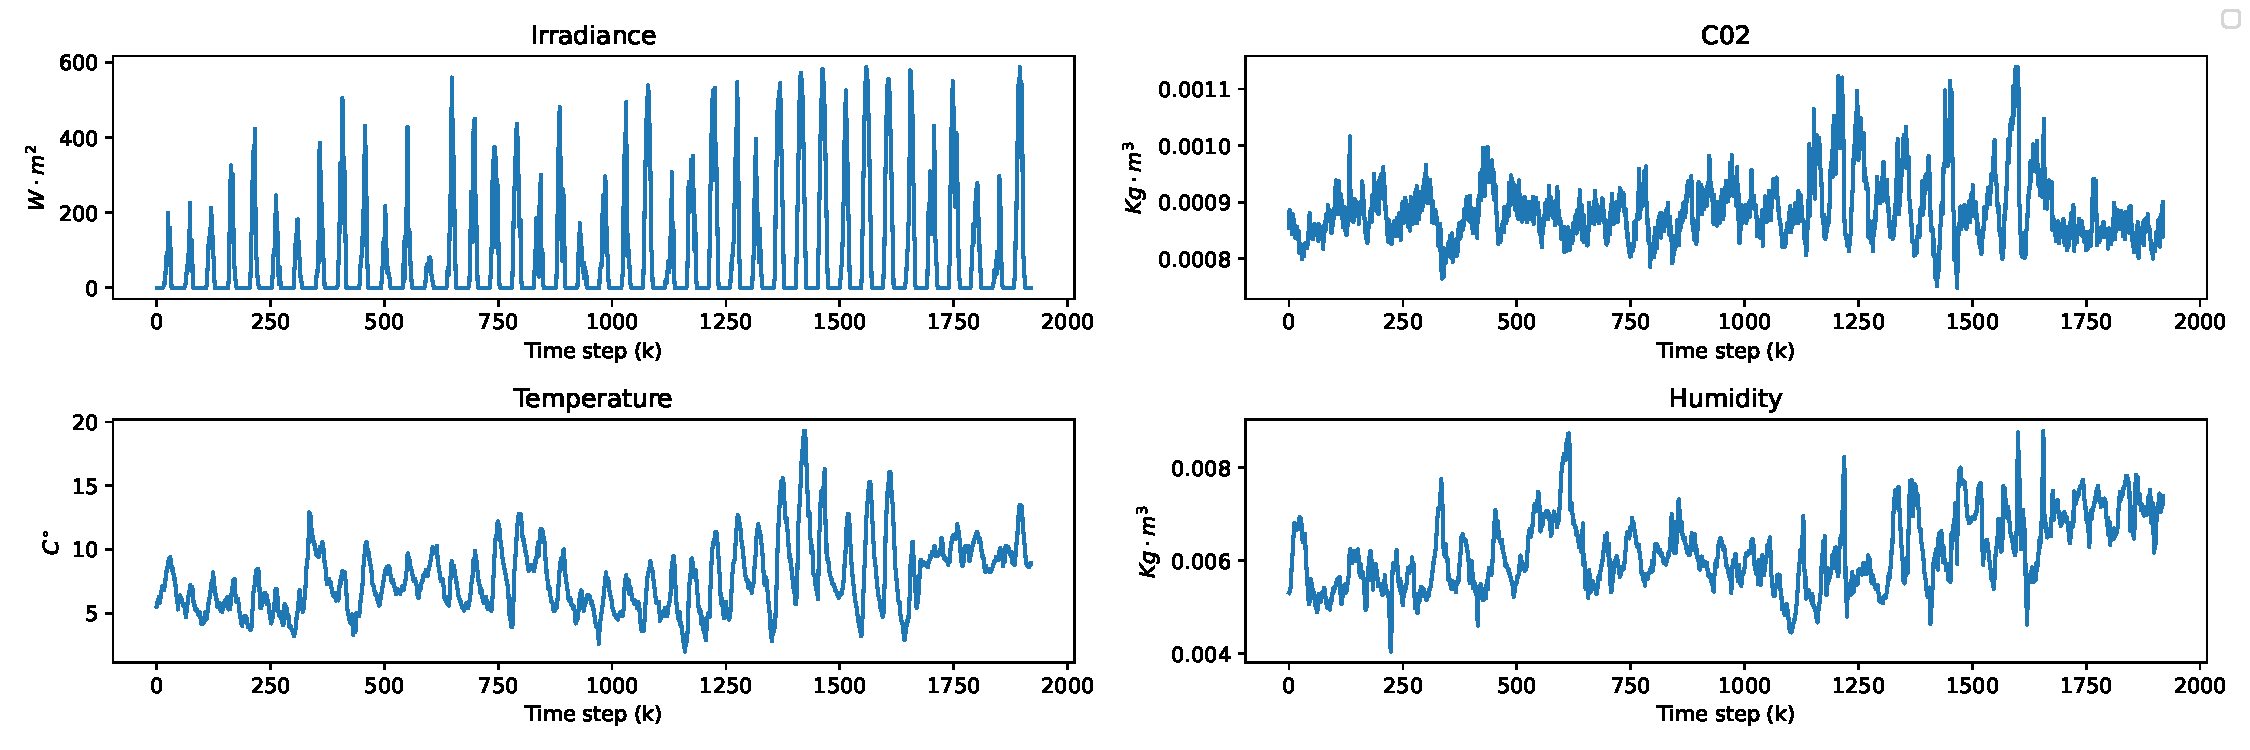
\includegraphics[width=\textwidth]{figures/weather_data.pdf}
    \caption{Weather Data}
    \label{fig:weather-data}
\end{figure}

The weather data used in training was obtained from the Venlow Greenhouse in Bleiswijk from January 30–March 11, 2014. The weather data was resampled from its original 5-minute interval to a 30-minute interval following the timestep of the environment. The weather data remains consistent throughout the episodes, irrespective of whether the training and evaluation is conducted under deterministic or stochastic conditions since it is not important to have the agent generalize well across various weather patterns in this thesis. Therefore, the validation data is the same as the training data, i.e. the same weather data is used in training as well as evaluating the agents performance. In practice, it may be necessary to evaluate the agent on unseen weather data to determine how well it is able to generalize to weather patterns. However, provided that all algorithms/controllers use identical weather data, it can be considered a suitable basis for comparing algorithms if the agent learns a suitable policy for this specific weather pattern.


\paragraph{Deterministic and Stochastic Environment}
When learning a policy in stochastic and deterministic environments, the key distinction lies in the evolution of the state of the greenhouse. In the stochastic case, this evolution follows the principles outlined in \autoref{eq:uncertainty_model}. In the stochastic setting, three agents were trained, each on a different level of uncertainty, namely $\delta = 5\%$, $\delta = 10\%$ and $\delta = 20\%$. While these uncertainty levels may seem extreme, learning a policy for each level was necessary to facilitate a easy comparison with MPC and RL-MPC under identical conditions. The choice of hyper parameters and neural network architecture that produce the most favourable policy in the deterministic setting will be used in the stochastic setting, thus there is no reevaluation of hyperparameters. While the stochastic environment represents a scenario closer to real-life conditions, the deterministic case offers a nominal measure of the RL agent's and MPC's performance and facilitates the development of the RL-MPC algorithm. The nominal case also serves whether the RL agent can provide suitable terminal constraints and cost function to the MPC for increased performance.

\paragraph{Performance Metrics}
The primary performance metric for evaluating RL agents is the final cumulative reward obtained over the 40-day growing period, i.e. the summation of \autoref{eq:reward_fn} over an episode. The performance metric under consideration is conceptually equivalent to the EPI (\autoref{eq:epi}) minus the summed temperature, $CO_2$ and humidity violations. This is a natural selection of the final performance metric as it directly corresponds to what the RL agent, MPC and RL-MPC controllers are optimising. Other metrics include the EPI, total growth, total $CO_2$ usage, total heating, computational time to compute control input, temperature and $CO_2$ violations. It is difficult to compare these lesser performance metrics across policies since they all form part of the reward function (except the computational time) and are not directly optimised. Therefore, comparisons would be meaningless, and only observations can be made. However, the computational time to compute the optimal control action is an important metric, particularly when combining RL with MPC. Finally, when comparing the controllers in a stochastic environment, the variance of the final cumulative reward is also examined. Although variance is not optimised, it serves as a measure of robustness of the resulting agent in a stochastic environment.

\section{Hyper-parameter Tuning}
Hyper-parameter tuning is frequently laborious and requires exhaustive exploration to determine the best configuration for a policy that maximises the cumulative reward of the agent. Therefore, the final hyper-parameters are posted in \autoref{tab:hyper-params} and were found empirically. The discount factor and activation function are not reported here, since they are further discussed in \autoref{ssection:discount-factor} and \autoref{ssection:act-fn} respectively. The effect of these two parameters is important to consider when integrating the value function of the learned agent with MPC. The defaults provided by SB3 are used for hyper-parameters that are not reported.

\begin{table}[H]
	\centering
	\renewcommand{\arraystretch}{1.3} % Adjust row height
	\begin{tabular}{|c|c|}
		\hline
		\textbf{Parameter} & \textbf{Value} \\
		\hline
		Training episodes & $100$  \\
		Warm-up episodes &  $9$\\
		Hidden layers & $2$ \\
		Neurons per hidden layer & $128$ \\
		Batch size & $1024$ \\
		Learning rate & $5 \cdot 10^{-3}$ \\
		Buffer size & $100,000$ \\
		\hline
	\end{tabular}
	\caption{Hyper-parameters}
	\label{tab:hyper-params}
\end{table}


\paragraph{Activation Function} 
The importance of the activation function lies in whether the resulting activation allows the output of the neural network to be differentiable with respect to the inputs. For instance, the ReLu activation function is commonly used due to its simplicity and superior convergence. Although ReLu is differentiable concerning the weights of the neural network, it is not differentiable to the inputs of the neural network. This is important to note since the trained value function must be differentiable with respect to its inputs if it is to be used as a cost function in the MPC formulation. Hence, the tanh function may be used instead, as it is a frequently used activation function that is differentiable concerning the inputs.

\paragraph{Discount Factor} 
Another consideration is the discount factor, denoted as $\gamma$. In RL problems with a fixed, long-term horizon, a discount factor ($\gamma$) of 1 is often desired. This setting ensures that the RL agent's prediction horizon covers the entire growing period, allowing the critic to evaluate and retain information about the full state trajectory and the actor to make long-term decisions, which is highly desirable for optimising economic benefits. Having $\gamma < 1$ will shorten the agent’s ‘prediction horizon’, and the resulting value function may not provide significant benefits for the MPC when integrated. However, it may stabilise the learning and yield a better policy than when $\gamma = 1$, due to the decrease in complexity of the problem. Results of the activation function and discount factor are shown and discussed in \autoref{section:rl-deterministic-results}.

\section{Deterministic Results}
This section presents and examines the outcomes of modifying the discount factor and the activation function. Finally, a discussion of the chosen policies and identifying the desirable characteristics that can be integrated with the MPC is performed. While several hyperparameters can impact the performance of the resulting RL policy, this section will focus on the discount factor and activation function. These two parameters are considered necessary aspects of the RL policy, particularly when it is desired to integrate it with MPC.

\subsection{Discount Factor}\label{ssection:discount-factor}
Typically, the discount factor lies between 0.9 and 0.99. Economic optimisation should have this discount factor as close to 1 as possible. Therefore, four discount factors were tested, namely 1, 0.99, 0.95 and 0.9. Going any lower may yield a more stable learning procedure at the cost of a more myopic policy. It should be noted that the ReLu activation function was used for the following results as it was found to display quicker and more stable learning of the policy than the tanh function. The value functions trained on their respective discount factor are denoted $V_{\pi|\gamma}(s)$.

\begin{figure}[H]
	\centering
	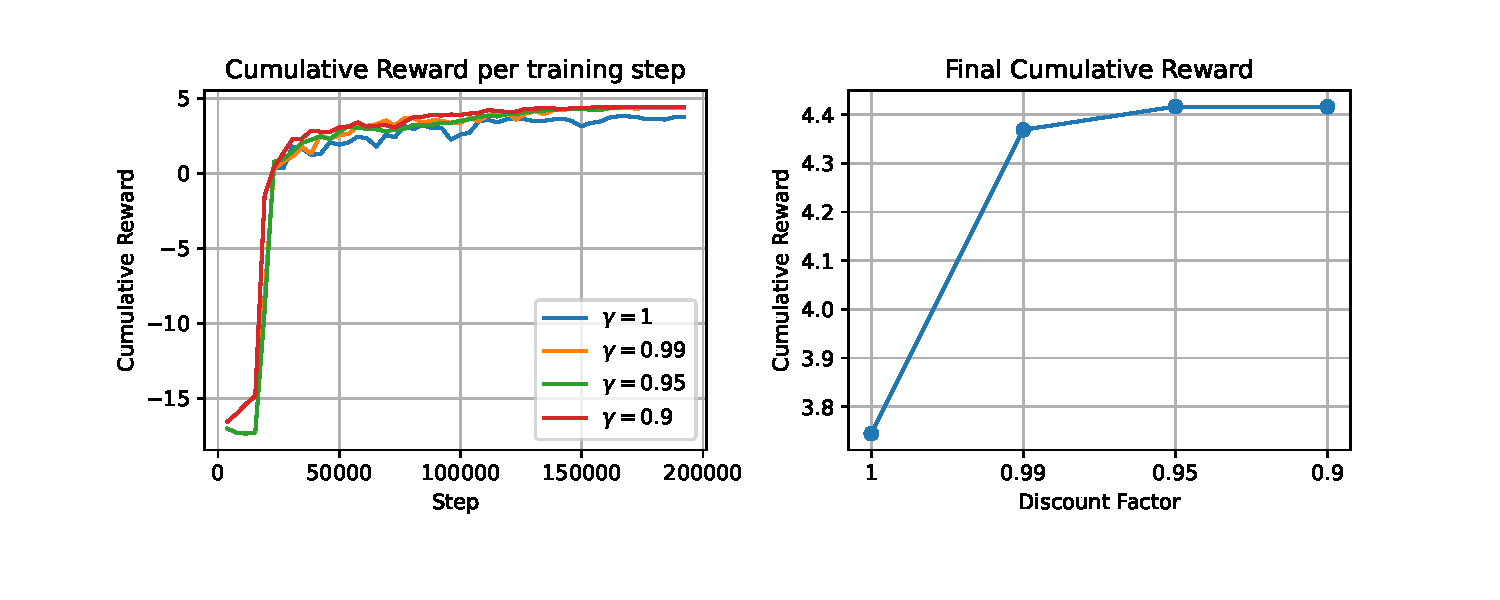
\includegraphics[width = \textwidth]{figures/gamma_reward.pdf}
	\caption{Cumulative reward vs discount factor ($\gamma$)}
	\label{fig:gamma_vs_reward}
\end{figure}

\paragraph{Policy Performance} 
The cumulative reward achieved as the policy is trained and the final cumulative reward after training for each different discount factor is depicted in \autoref{fig:gamma_vs_reward}. The cumulative reward per training step is an example of the learning process, while the final cumulative reward depicts the final performance of the RL agent. As seen in \autoref{fig:gamma_vs_reward}, it is clear that $\gamma = 1$ does not perform as well as lower discount factors. It is noted that the degradation in performance comes from the increase in problem complexity when the discount factor is 1. Hence, it becomes increasingly more difficult to find an optimal policy, one that might require a different set of hyper-parameters and potentially a significantly larger number of training episodes. However, the policy generated with this discount factor will provide a value function that holds information across the entire time horizon, which is desirable. Conversely, the learning procedure is much more stable when lower discount values are used, and thus, a higher final cumulative reward is achieved. Nevertheless, this adjustment means that the critic's value estimates are based on discounted returns rather than the true long-term expected return. Given the desirability of using the value function in the MPC formulation, it is necessary to analyse the value function for each tested discount factor.


\paragraph{Value Function}
It is difficult to determine whether the critic has converged. Given that the critic serves as a Q-value function approximator in the SAC algorithm, the actor must identify the optimal action for a given state to compute the value of that state using the critic. Therefore, convergence of the value function is also dependent upon the actor policy. Although the training curves indicate that the critic has converged, it has only converged in alignment with the actor’s policy. It is necessary to visualise and compare the actual (computed by \autoref{eq:total-return} through simulating the policy) and the predicted value (given by the learned value function) of a given visited state during the 40-day simulation to assess whether the critic (and actor) have achieved convergence in predicting the value function. In addition, \autoref{eq:v0} may be used as a visual aid to compare the accuracy of the learned value function ($V_{\pi|\gamma}(\cdot)$) to a non-discounted value function, i.e. $\gamma = 1$ ($V_{\pi|\gamma=1}(\cdot)$).
\begin{equation}\label{eq:v0}
	\begin{aligned}
		V_{\pi|\gamma = 1}(s_k) &= r_k + V_{\pi|\gamma = 1}(s_{k+1}) \\
		\therefore V_{\pi|\gamma = 1}(s_{k-1}) &= r_{k-1} + V_{\pi|\gamma = 1}(s_{k}) \\
		\therefore V_{\pi|\gamma = 1}(s_{k-2}) &= r_{k-2} + r_{k-1} + V_{\pi|\gamma = 1}(s_{k}) \\
		\therefore V_{\pi|\gamma = 1}(s_{0}) &= \sum_{i=0}^{k-1} {r_{i}} + V_{\pi|\gamma = 1}(s_{k})   \\
	\end{aligned}
\end{equation}

During each time step and using \autoref{eq:v0}, the state’s non-discounted value is computed by the cumulative rewards received up to that point and the approximation of the current state’s value using the learned value function. If a value function can approximate the non-discounted value of a state accurately, then \autoref{eq:v0} should yield the same result for every time step, resulting in a horizontal line, $y = V_{\pi|\gamma = 1}(s_0)$. It is noted, that only a value function trained on $\gamma = 1$ would be able to achieve this; however, it serves as an important visual aid to show the accuracy of the trained value functions.

For each discount factor and at each time step for the 40-day growing period the following were plotted and is shown in \autoref{fig:vf-vs-gamma}: the predicted discounted value of each state visited (as predicted by the learned $V_{\phi|\gamma}$), the predicted initial non-discounted value (as predicted by \autoref{eq:v0}), the cumulative rewards obtained (recorded during the simulation) and finally the actual value of a state (calculated from the cumulative rewards and \autoref{eq:total-return}). For the deterministic case, the realisations of state trajectories and rewards received do not differ between simulations. Hence, the exact value of each state may be calculated. 

\begin{figure}[H]
    \centering
    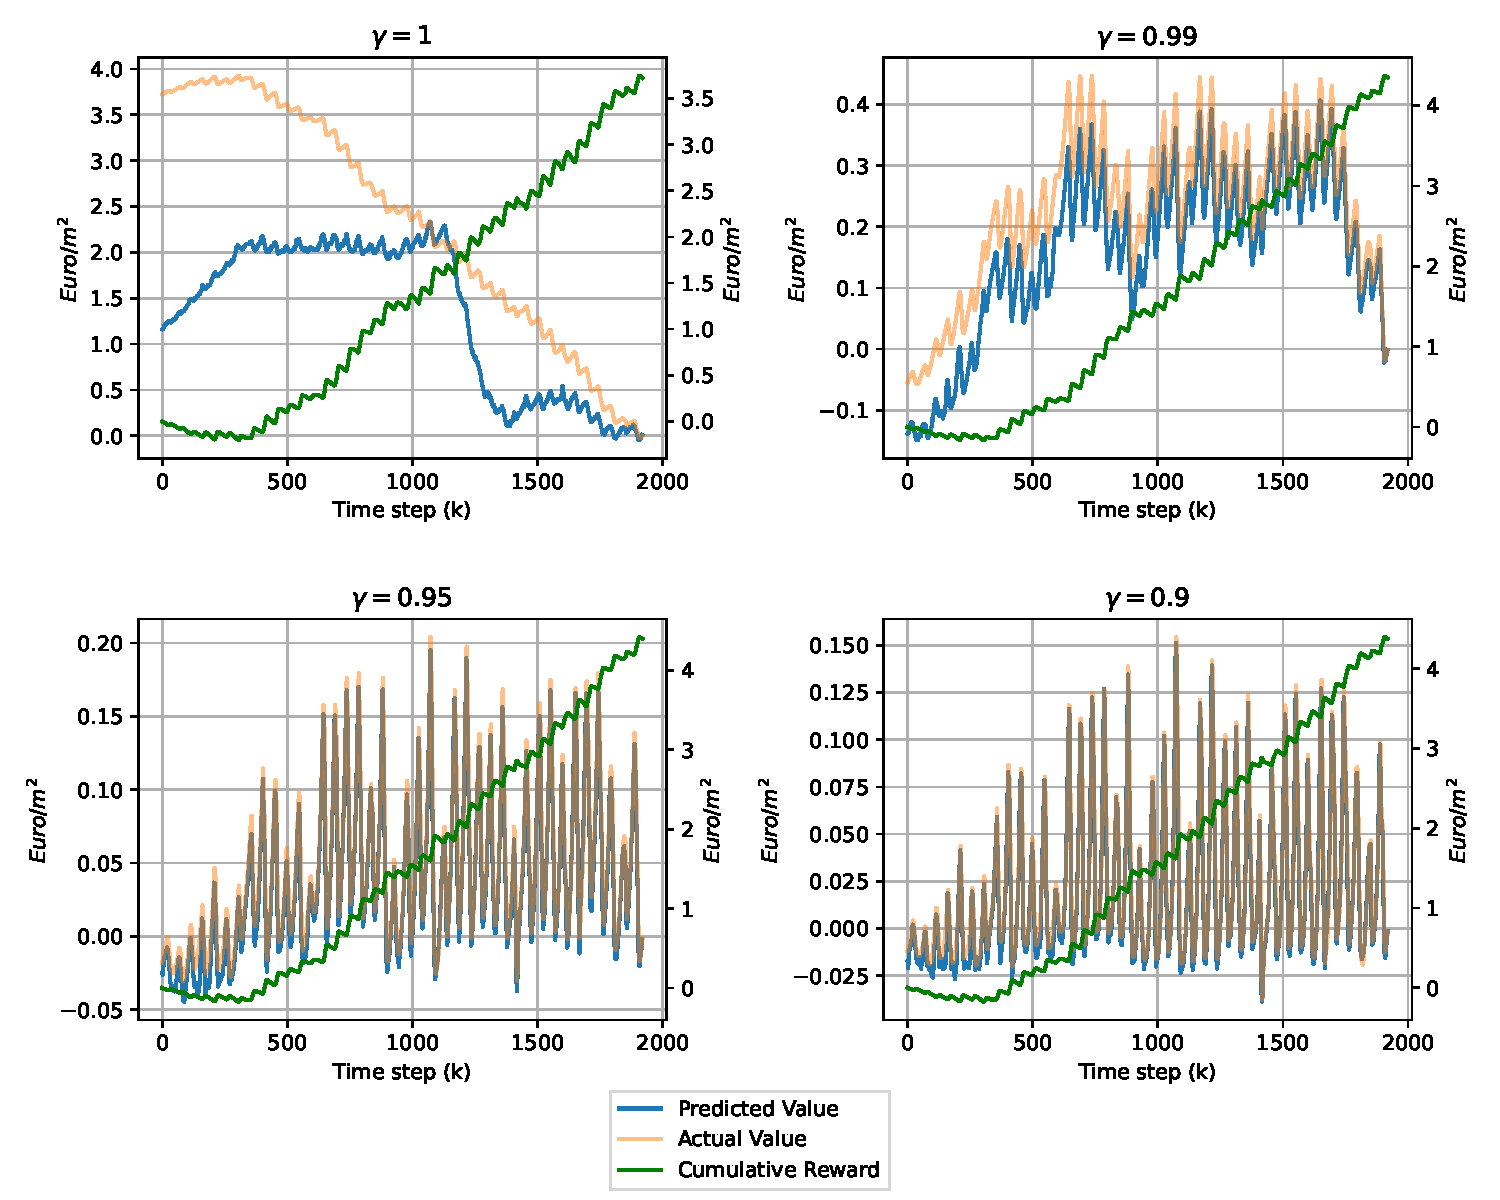
\includegraphics[width = \textwidth]{figures/vf_vs_gamma.pdf}
    \caption{Predicted value vs actual value vs discount factor}
    \label{fig:vf-vs-gamma}
\end{figure}

 Naturally, as seen in \autoref{fig:vf-vs-gamma} the cumulative reward differs slightly between discount factors since the policy generated is also dependent on the value function obtained. It is noted that the trajectory of the actual value (for $\gamma = 1$) is a horizontally reflected trajectory of the cumulative rewards trajectory which is aligned with the definition of a value function (\autoref{eq:value_function}) and can be seen in \autoref{fig:vf-vs-gamma}. Naturally, this is not the case for discount factors lower than one since the value only embeds knowledge of future rewards to be received over a shorter horizon. This is further seen by the predicted $V_{\pi}(s_0)$, whereby the value functions do not produce a horizontal $V_{\pi}(s_0)$ curve, indicating their inadequacy in predicting the true non-discounted value function (as expected since they were trained on discounted rewards). One would expect that only $V_{\pi}(s|\gamma = 1)$ should be able to predict a non-discounted value (since it was trained on non-discounted rewards), however; it is evident that not even $V_{\pi}(s|\gamma = 1)$ is able to do this, as shown by the clear non-horizontal predicted $V_{\pi}(s_0)$ curve. This is most likely due to the increased problem complexity, which makes accurate approximations of the value difficult when trained with $\gamma = 1$.
 
It is also noted that the lower the discount factor, the more accurate the predicted discounted-value of a state becomes, as seen by the overlapping ‘predicted’ and ‘actual value’ curves. This may be due to decreased problem complexity and more accurate approximations. When $\gamma = 0.9$, the critic is capable of accurately predicting the actual discounted value of a state. However, as mentioned, it falls short of accurately representing the true non-discounted value of a state. The same can be said for all discount factors lower than one. It was important to train an actor and critic with a $\gamma = 1$ because it was believed that despite the worse performing policy, the trained critic would still provide a reasonable estimation of the non-discounted value of a state. When examining \autoref{fig:vf-vs-gamma}, it becomes evident that this assumption is incorrect. During the investigation into suitable hyper-parameters for the learning agent, it was observed that when $\gamma = 1$, the trained critic struggled to estimate the value of a state in all cases accurately. \autoref{fig:vf-vs-gamma} is just one such realisation.

\subsection{Activation Function}\label{ssection:act-fn}
It is also important for the trained critic to use differentiable activation functions to ensure differentiability. This is done so that it may be used in the MPC framework. However, an activation function, such as the commonly used tanh activation, may or may not yield desirable results in maximising cumulative reward. This section compares the performance (final cumulative reward) of a learned agent with tanh activation functions against agents with ReLu activation functions for a $\gamma = 1$ and $\gamma = 0.95$, with the ReLu acting as the baseline performance.


	
\begin{table}[h!]
	\centering
	\begin{tabular}{c c c c}
		\toprule
		\multirow{2}{*}{\textbf{Discount Factor}} & \multicolumn{2}{c}{\textbf{Performance}} & \multirow{2}{*}{\textbf{Performance Increase (\%)}} \\
		\cmidrule{2-3}
		& \textbf{ReLU} & \textbf{tanh} &  \\
		\midrule
		\textbf{1}   & 3.72 & 3.44 & -7.53 \\
		\textbf{0.95} & 4.27 & 4.17 & -2.34 \\
		\bottomrule
	\end{tabular}
	\caption{ReLu vs Tanh on performance with ReLu as baseline performance}
	\label{table:tanh-act-fn}
\end{table}
	
\autoref{table:tanh-act-fn} displays the effect of the tanh activation on the agent’s final performance. It is clear that ReLu outperforms the tanh activation function in terms of final cumulative reward. This situation presents a dilemma. It is desirable to have an effective RL policy in which the critic has differentiability. While additional investigation into the hyper-parameters may be necessary to improve the perfomance when using tanh activation functions, the focus of this thesis does not lie in developing the best possible RL-generated policy. Instead, this chapter aims to develop an RL policy comparable to MPC, along with an accurate critic. The focus of these results is to make clear the obstacles in developing an appropriate actor and critic to be used in the RL-MPC framework.

\subsection{Final Results and Conclusion}
\label{section:rl-deterministic-results}

From the findings, the best policy produced by RL is with the hyper parameters shown in \autoref{tab:hyper-params}, with a $\gamma = 0.95$  and with ReLu activation functions. While the best-performing policy is desired, this configuration does not produce adequate conditions for its critic to be used in the MPC formulation; namely, the value function does not hold information across the entire prediction horizon and is not differentiable. An agent learned with a $\gamma = 1$ and tanh activation function, results in a worse performing policy and a critic that struggles to predict the value of states accurately. With that being said, a critic that has undergone training with a discount factor of $\gamma = 0.95$ is able to accurately predict the discounted-value of a state and may still possess sufficient knowledge regarding future rewards to be advantageous for MPC. Additionally, a critic learned with a $\gamma = 1$, albeit bad approximations, may also provide enough information about future rewards. To reconcile these issues, a separate critic was trained with $\gamma = 1$ on the fixed best-performing policy. This approach leverages the advantages of a practical policy while ensuring that the critic provides accurate value estimations over the entire trajectory. 

\begin{table}[h!]
	\centering
	\begin{tabular}{c c c c}
		\toprule
		\textbf{Agent} & $\boldsymbol{\gamma}$ & \textbf{Activation Function} & \textbf{Final Performance} \\
		\midrule
		\textbf{ 1} & 0.95 & ReLU & 4.27 \\
		\textbf{ 2} & 0.95 & Tanh & 4.18 \\
		\textbf{ 3} & 1 & Tanh & 3.44 \\
		\bottomrule
	\end{tabular}
	\caption{Performance of agents with different activation functions and discount factors}
	\label{tab:selected_agents}
\end{table}

\begin{figure}[H]
    \centering
    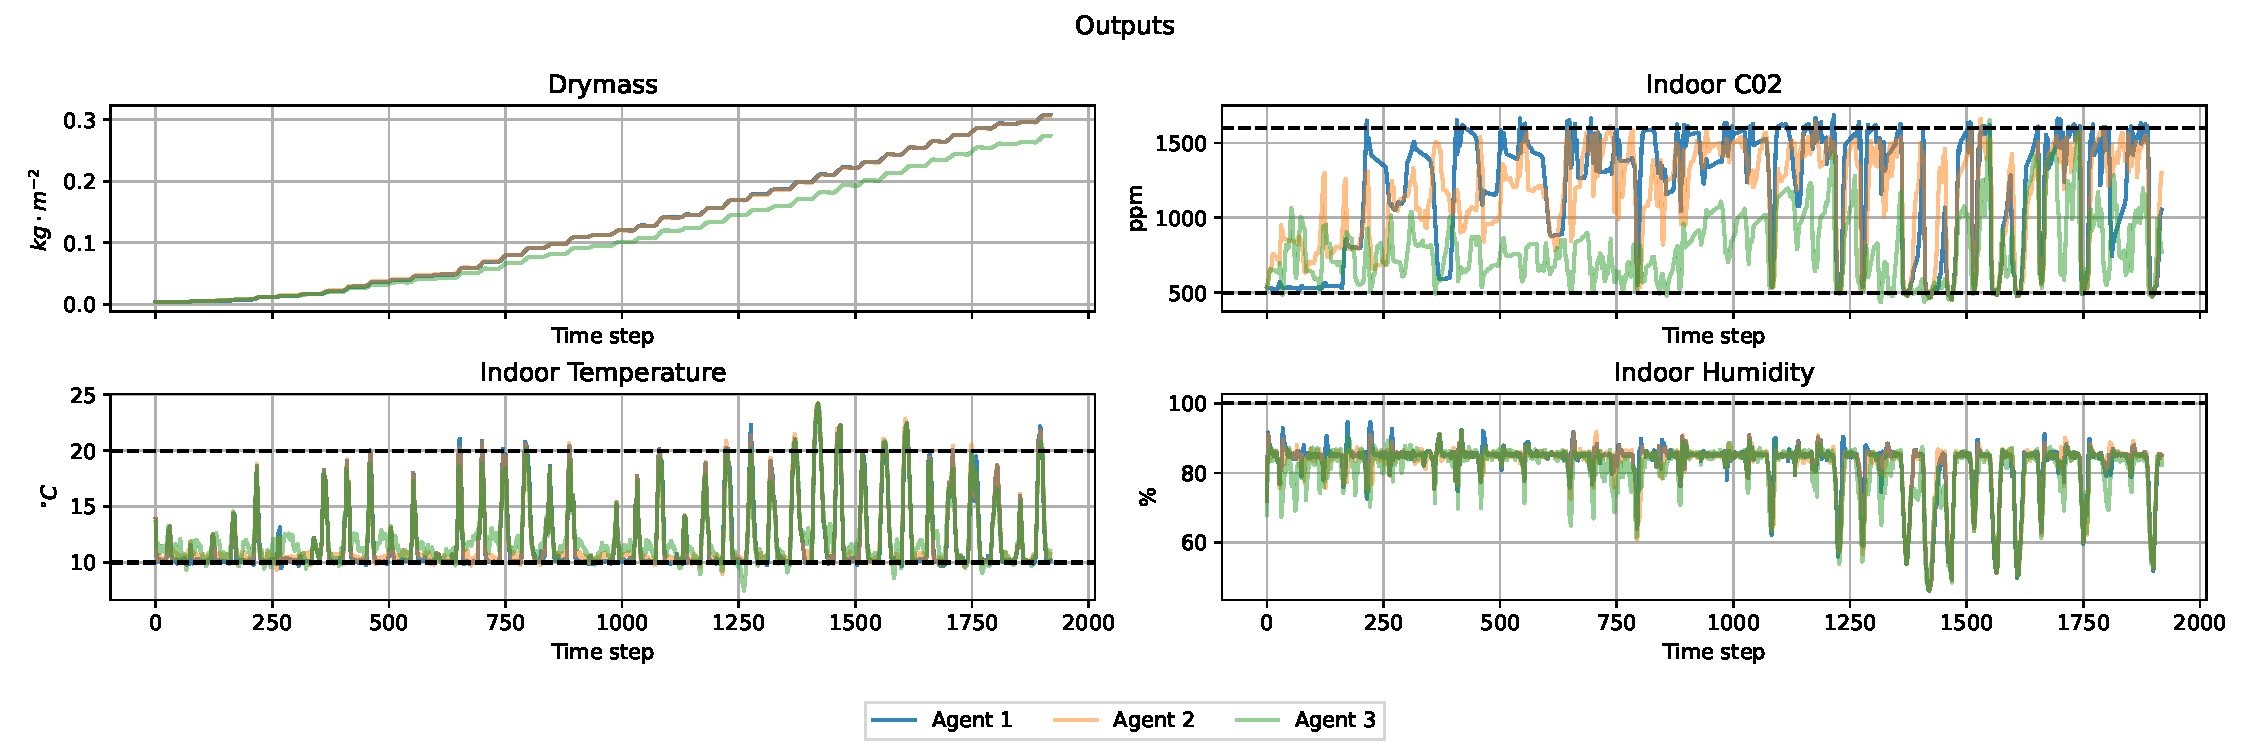
\includegraphics[width = \textwidth]{figures/selected_policies_outputs.pdf}
    \caption{Time series of system outputs}
    \label{fig:selected-policies-outputs}
\end{figure}

\begin{figure}[H]
    \centering
    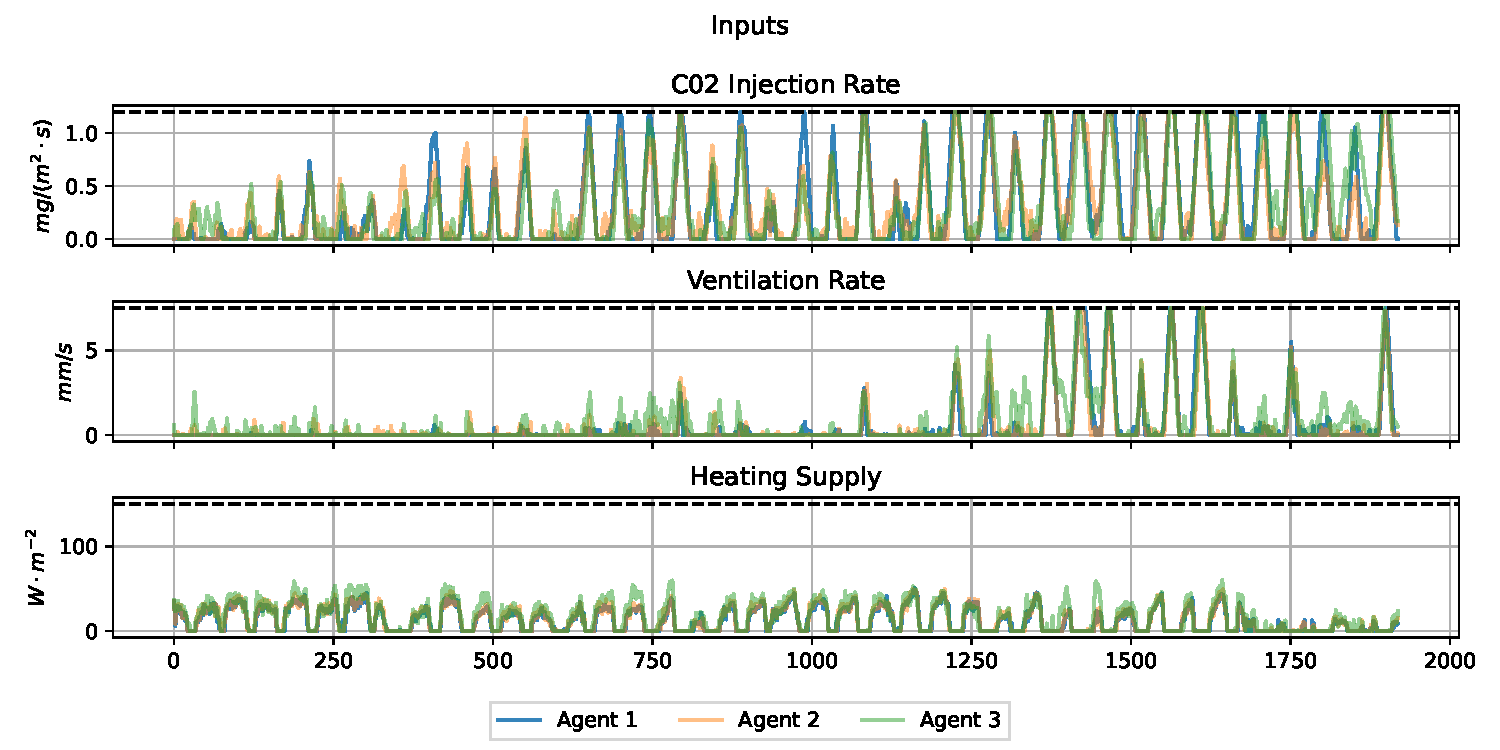
\includegraphics[width = \textwidth]{figures/selected_policies_inputs.pdf}
    \caption{Time series of system outputs}
    \label{fig:selected-policies-inputs}
\end{figure}

\autoref{tab:selected_agents} displays 3 agents each with differing activation functions or discount factor, whereby Agent 1 is the best policy obtained. The time series plot of the system outputs and inputs across the 40 days for every agent in \autoref{tab:selected_agents} is shown in \autoref{fig:selected-policies-outputs}. These time series plots are similar to those reported in \citet{jansenOptimalControlLettuce2023,morcegoReinforcementLearningModel2023}. Direct comparisons are not possible since \citet{morcegoReinforcementLearningModel2023} does not specify the weather data range used and the reward function differs from what is used in this thesis. Furthermore, \citet{morcegoReinforcementLearningModel2023} includes additional constraints on temperature levels during the day to encourage heating by solar radiation during the day and the heating system at night. This thesis did not include these constraints because the thesis aimed to give RL more independence in optimising EPI while minimising dangerous constraint violations for plant and/or human operation. Furthermore, \citet{jansenOptimalControlLettuce2023} also reports similar results; however, a direct comparison is not possible since hyper-parameters and reward functions differ. However, it is noted that results, time series and cumulative rewards are similar enough to give confidence in the correct setup and training of the RL agent.

\begin{table}[H]
	\centering
	\renewcommand{\arraystretch}{1.3} % Adjust row height
	\begin{tabular}{|c|c|c|c|}
		\hline
		\textbf{Metric} & \textbf{Agent 1} & \textbf{Agent 2} & \textbf{Agent 3} \\
		\hline
		EPI                & 4.964      & 4.807     & 3.727 \\
		Total Growth       & 0.304      & 0.303     & 0.270 \\
		Total CO2 Usage    & 1.057      & 1.0318    & 1.029 \\
		Total Heating      & 12.5462    & 13.661    & 16.381 \\
		Computational Time & 0.000216   & 0.00024   & 0.00023 \\
		Temp Violations    & 110.007    & 119.2     & 138.93 \\
		CO2 Violations     & 3311.43    & 1046.47   & 1972.61 \\
		Final Performance  & 4.27       & 4.173     & 3.031 \\ 
		\hline
	\end{tabular}
	\caption{Performance Metrics of Agents}
	\label{tab:perf-metrics-selected-policies}
\end{table}


Other performance metrics are reported for completeness in \autoref{tab:perf-metrics-selected-policies}. It is noted that the computational time needed to compute the control action takes $\approx 0.2ms$. This is expected since a simple inference of the actor network is required to calculate the action. Other metrics, as reported in \autoref{tab:perf-metrics-selected-policies}, may be useful when designing a controller specifically for a greenhouse where the total heating and $CO_2$ may provide additional insight. However, the RL-MPC controller developed in this thesis focuses on the economic optimisation of a system and is only concerned about the optimisation goal in \autoref{eq:optimisation-goal}.

\section{Stochastic Results} \label{section:rl-stochastic-results}
In training the stochastic RL agent, the same hyper-parameter configuration used to produce the best nominal agent, Agent 1 (\autoref{tab:selected_agents}), was used. Three stochastic agents were trained on a different level of uncertainty as specified in \autoref{section:env-description} with the uncertainty model according to \autoref{eq:uncertainty_model}. Performance metrics are reported, and a comparison is made with the nominal model (Agent 1 from \autoref{tab:selected_agents}). Performance metrics are evaluated by repeating the 40-day simulation period 30 times and taking the average and variance of the final cumulative reward over the growing period. Each agent is assigned a name based on the degree of uncertainty on which they received training. For example, an agent that has undergone training in a stochastic environment with a $\delta = 20\%$ is referred to as ‘Agent 0.2’. The nominal agent named ‘Agent 1’ is also referred to as the ‘nominal agent’. Every agent is compared to one another for every level of uncertainty.

\begin{figure}[H]
    \centering
    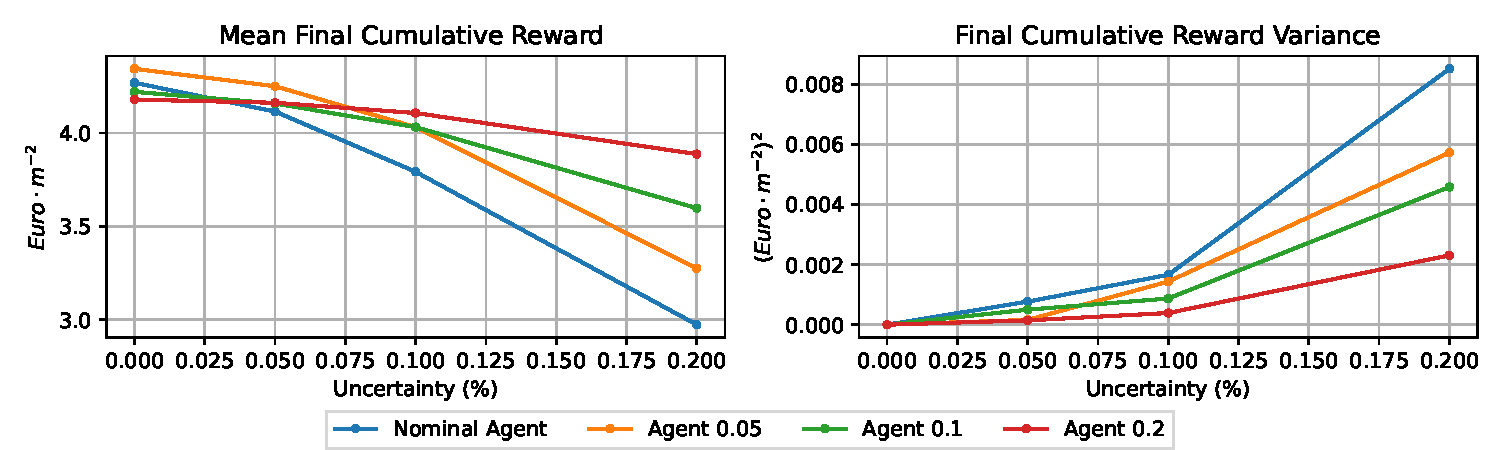
\includegraphics[width = \textwidth]{figures/stochastic_rl_policies.pdf}
    \caption{Stochastic RL policy performances}
    \label{fig:stochastic-rl-policies}
\end{figure}

The mean final cumulative reward and variance of each agent under different uncertainty levels are presented in \ref{fig:stochastic-rl-policies}. As expected, as more uncertainty is injected into the environment, the mean cumulative reward decreases and the variance increases. There is a noticeable trend where agents trained with higher levels of uncertainty tend to have a slower decline in performance as uncertainty increases. However, they may not perform as well at lower levels of uncertainty compared to agents trained with lower levels of uncertainty. Similarly, agents trained on higher uncertainty levels maintain a lower variance in their final cumulative reward as uncertainty increases, compared to agents trained on data with lower uncertainty. This is typical behaviour when comparing a more robust policy to a less robust policy.\\
Although, in practice, the uncertainty is not known, if a more robust policy is desired, training a RL agent on a higher level of uncertainty than expected may achieve the desired outcomes. Also, in general, the results also suggest that an agent trained on a level of uncertainty does not necessarily produce the best policy for that level of uncertainty. It seems that, in the nominal case ($\delta = 0\%$), the agent trained on a $5\%$ uncertainty level (Agent 0.05) outperforms the nominal agent. Moreover, Agent 0.2 seems to achieve a higher average cumulative reward than Agent 0.1 when tested on a $10\%$ uncertain model. It is anticipated that agents who are trained and tested based on their respective uncertainty would exhibit superior performance. However, this disparity in performance can be attributed to the agent’s increased exploration due to the added noise.

\subsection{Conclusion}
It is widely recognised that RL can address uncertainty by introducing this uncertainty in the training data, as evidenced by the findings presented in \autoref{fig:stochastic-rl-policies}. The incorporation of these stochastic policies into the MPC framework will be examined to determine whether an RL policy learned from stochastic data can transfer its characteristics to the RL-MPC framework. Finally, each agent, specifically the nominal agent, Agents 0.05, 0.1 and 0.2, are used in its corresponding stochastic environment. Although Agent 0.05 may outperform the nominal agent under nominal conditions, each stochastic environment uses its corresponding agent when integrated into the RL-MPC framework. Moreover, due to the problematic critic (discussed in \autoref{section:rl-deterministic-results}) a separately trained critic with a discount factor of 1 was trained for each policy as was done in the nominal case.

\section{Trained Value Function}
\label{section:trained-vf}
Although training an agent using SAC produces an actor and a critic network, it was shown in \autoref{section:rl-deterministic-results} that the produced critic had undesirable characteristics. This critic was continually trained based on a changing policy dependent on the critic itself; therefore, it is not surprising that the approximation to the value function was sub-optimal. However, this section aims to train a value function (using a neural network as a function approximator) with a fixed policy \footnote{This fixed policy may come from any control lay, however the RL policy is used due to its computational efficiency in determining control actions, enabling large amounts of data points and/or trajectories to be obtained}. Therefore, a value function may be trained on the best policy obtained. Additionally, there is more freedom in choosing the architecture of the value function since it is now trained independently of the policy. Therefore, simpler models may be made and tested to approximate the value function. Specifically, upon inspection of \autoref{fig:selected-policies-outputs} and \autoref{fig:vf-vs-gamma}, it is noticed that the cumulative reward at each time step primarily depends on the state of the crop’s dry mass at time $k$. Therefore it may be possible to learn a value approximator solely based on the crop’s dry mass and current time. Lastly, the tanh activation functions must be used to ensure differentiability. Two methods were employed to learn various value function approximators: the temporal difference learning method and the expected return method, each with their respective advantages and disadvantages. It is noted that this value function is only accurate under the policy on which it was trained. A value function is trained for the nominal agent and each stochastic agent, however data acquisition and value function training will be explained for the nominal agent as it is identical for the stochastic agents.


\subsection{Temporal Difference Learning}
\label{ssection:td-learning}

This method uses a similar technique by which SAC, DDPG and TD3 update their critic. Two neural networks represent the value function, a current and a target network. The mean squared Bellman error is minimised between the target values (from the target network) and the current values (from the current network), as shown in \autoref{eq:vf_td_loss}. Moreover, Polyak averaging is used to update the target networks. This method is very sample-efficient compared to the expected return learning. As a result, it will be easier to cover a wider range of states in the sampled state space. Consequently, the method is effective in learning a value function that can effectively generalise across the entire state space. 

\paragraph{Obtaining Data}
The nominal agent (Agent 1 from \autoref{tab:selected_agents}) was used to acquire the data. A similar methodology for data acquisition as described in \citet{linReinforcementLearningBasedModel2023} was employed. Along the nominal trajectory, $q$ ($q \in \mathbb{N}_{>0}$) internal states, $x$ and inputs $u$, were uniformly sampled from $\hat{\mathbb{X}}^4$ (\autoref{eq:td_state_space}) and ${\mathbb{U}}^3$ (\autoref{eq:constraints}) at time $k$ respectively. So that at time $k$, a set denoted as $\hat{S}_{k} = \{\hat{s}_{k_1},\hat{s}_{k_2},...,\hat{s}_{k_q}\}$ is created, where $\hat{s}_{k_i}$ is constructed using \autoref{eq:obs-tuple-1} from the sampled states and inputs. Each element in $\hat{S}_k$, denoted $\hat{s}_{k_i}$, is taken separately as an initial state and evolved one step in time with the RL agent, receiving a reward $\hat{r}_{k_i}$ and a Boolean $d$ indicating whether a terminal state has been reached. $\hat{s}_{k_i}$ and $\hat{s}_{{k+1}_i}$ are both normalised as per \autoref{eq:state-normalization} and stored in a transition tuple along with the received reward and $d$, denoted as $(\hat{s}_{k_i},\hat{s}_{{k+1}_i},\hat{s}_{k_i},d)$. The environment is then set back to the actual state $s_k$ and evolved for one time step, and the process repeats itself, until the 40 days are over. The transition tuple of the actual system is also stored. The quality of sampled internal states and inputs is important to ensure that a value function approximator generalises well across the state space. \\
From the time series plots \autoref{fig:selected-policies-outputs} and \autoref{fig:selected-policies-inputs}, it can be seen that not the entire state space needs to be sampled, especially for the dry mass state, $x_1$. The control actions were sampled across the entire control space $\mathbb{U}^3$ as shown in \autoref{eq:constraints}. States $x_2,x_3,x_4$ were sampled with a range slightly larger than their respective minimum and maximum constraints (\autoref{eq:constraints}) range. This decision was made as it was deemed unnecessary to sample states that significantly violate constraints. Finally, $x_1$ was sampled around the nominal $x_1$ trajectory such that the sampled state space $\hat{\mathbb{X}}^4$ is defined as:



\begin{equation}\label{eq:td_state_space}
\begin{split}
\hat{\mathbb{X}}^4 = \{ (\hat{x_1}, \hat{x_2}, \hat{x_3}, \hat{x_4}) \mid\ & \hat{x_1} \in [\hat{x}_{1\min}(x_{1_k}), \hat{x}_{1\max}(x_{1_k})], \\
& \hat{x_2} \in [\hat{x}_{2\min}, \hat{x}_{2\max}], \\
& \hat{x_3} \in [\hat{x}_{3\min}, \hat{x}_{3\max}], \\
& \hat{x_4} \in [\hat{x}_{4\min}, \hat{x}_{4\max}] \}
\end{split}
\end{equation}
where the bounds are specified in \autoref{tab:sample_bounds_td} and were found empirically and $\hat{x}_i$ denotes the sampled state and $x_{1_k}$ denotes the nominal dry mass state at time $k$. It is noted that the bounds of the sampled state space (\autoref{tab:sample_bounds_td}) is specified in units used for the output variables, although it is easily converted to the correct units as used by the model states by using the inverse of the output equations (\autoref{eq:output_equations_c02} and \autoref{eq:output_equations_h}).

\begin{table}[H]
	\centering
	\begin{tabular}{|c|c|c|}
		\hline
		\textbf{Parameter} & \textbf{Value} & \textbf{Unit} \\
		\hline
		$\hat{x}_{1\min}(x_{1_k})$ & $x_{1_k} \cdot (1 - 0.8) - 0.01$ & $kg \cdot m^{-2}$ \\
		$\hat{x}_{1\max}(x_{1_k})$ & $x_{1_k} \cdot (1 + 0.7) + 0.01$ & $kg \cdot m^{-2}$ \\
		$\hat{x}_{2\min}$ & $g_{CO_2}^{-1} (\hat{x}_{3_k}, 400)$ & $ppm$ \\
		$\hat{x}_{2\max}$ & $g_{CO_2}^{-1} (\hat{x}_{3_k}, 1800)$ & $ppm$ \\
		$\hat{x}_{3\min}$ & $7$ & $^\circ C$ \\
		$\hat{x}_{3\max}$ & $30$ & $^\circ C$ \\
		$\hat{x}_{4\min}$ & $g_{h}^{-1} (\hat{x}_{3_k}, 50)$ & $RH_{\%}$ \\
		$\hat{x}_{4\max}$ & $g_{h}^{-1} (\hat{x}_{3_k}, 100)$ & $RH_{\%}$ \\
		\hline
	\end{tabular}
	\caption{Sample State Space Bounds}
	\label{tab:sample_bounds_td}
\end{table}


With only 10 additional samples every time step ($q=10$), the desired state space can be adequately covered.

\begin{figure}[H]
	\centering
	\includegraphics[width = \textwidth]{figures/sampled_y_td.png}
	\caption{Sampled States for Temporal Difference}
	\label{fig:sampled-states-TD}
\end{figure}
\begin{figure}[H]
	\centering
	\includegraphics[width = \textwidth]{figures/sampled_u_td.png}
	\caption{Sampled Inputs for Temporal Difference}
	\label{fig:sampled-inpts-TD}
\end{figure}

\autoref{fig:sampled-states-TD} and \autoref{fig:sampled-inpts-TD} display the states and inputs sampled during a 40-day period, respectively, with an additional ten samples taken at each time step, resulting in a total of $21120$ data points or transition tuples.



\paragraph{Training}
Once data is generated, it is split into a validation and training dataset with a 20\% and 80\% split respectively to ensure that the neural network does not overfit to the seen data. Transition tuples are sampled from the training set, and the following loss function is minimised:

\begin{equation}\label{eq:vf_td_loss}
    L(\phi, \mathcal{D}) =  V_{\phi}(s_k) - (r_k + (1-d) V_{\phi_{targ}} (s_{k+1}))
\end{equation}

where  $\phi$ and $\phi_{targ}$ are the current and target weights of the respective neural networks, and $\mathcal{D}$ is the training data set. The Adam optimiser minimises \autoref{eq:vf_td_loss} over a batch size $\mathcal{B}$. The target weight $\phi_{targ}$ are updated every learning iteration by Polyak averaging $\phi$:

\begin{equation}
    \phi_{targ} \leftarrow (1 - \rho) \phi_{targ} + \rho \phi
\end{equation}

where $\rho$ represents the Polyak coefficient, a hyper-parameter that needs to be tuned. Despite its widespread usage, it was discovered that the learning of the value function was consistently unstable regardless of the chosen hyper-parameters. It failed to learn an appropriate value function, but further research can be conducted to make it functional. However, stable learning was not attained in our work.

\subsection{Expected Return Learning}
This method includes obtaining the expected return of each state visited from a simulated trajectory under a fixed policy. The expected return can then be used as target values for a neural network to learn a value function approximator. Compared to the temporal difference learning method, this approach offers the benefit of considerably more stable training. Unlike the TD method, the targets remain unchanged while the weights of the neural networks are updated. However, this learning method is much less sample efficient, requiring significantly more data to generalise across the state space. Many trajectories are simulated until termination, and the return must be calculated for each state visited. More importantly, only the starting states of the trajectory are sampled, which makes it harder to obtain the same data spread as the TD method.

\paragraph{Obtaining Data}
A greater number of starting points must be sampled to obtain a spread comparable to the TD method; however, a significantly larger amount of data is needed because the trajectory must be run through to the end of the simulation. For each state visited, the expected return is calcualted using \autoref{eq:total-return}. Given the inferior sample efficiency of this method, it is important to carefully choose the starting states to ensure that the learned value function can effectively generalise across the state space that the agent is likely to encounter during a growing period. In selecting these initial states, a similar approach to \autoref{ssection:td-learning} was used. However, all initial states and inputs were uniformly sampled around a region of the nominal trajectory at time $k$ and not only the dry mass, $y_1$. Therefore, initial states and inputs were sampled from $\hat{\mathbb{X}}^4$ and $\hat{\mathbb{U}}^3$ and the initial time step $k$ is uniformly sampled across the entire time horizon as shown in \autoref{eq:TR-sample-space}.

\begin{equation}\label{eq:TR-sample-space}
\begin{split}
	& k \sim U(t_s,t_f)  \\
    \hat{\mathbb{X}}^4 &= \{ (\hat{x}_1, \hat{x}_2, \hat{x}_3, \hat{x}_4) \mid\ \hat{x}_1 \in [\hat{x}_{1\min}(x_{1_k}), \hat{x}_{1\max}(x_{1_k})], \\
    &\quad \hat{x}_2 \in [\hat{x}_{2\min}(x_{2_k}), \hat{x}_{2\max}(x_{2_k})], \\
    &\quad \hat{x}_3 \in [\hat{x}_{3\min}(x_{3_k}), \hat{x}_{3\max}(x_{3_k})], \\
    &\quad \hat{x}_4 \in [\hat{x}_{4\min}(x_{4_k}), \hat{x}_{4\max}(x_{4_k})] \} \\
    \hat{\mathbb{U}}^3 &= \{ (\hat{u}_1, \hat{u}_2, \hat{u}_3) \mid\ \hat{u}_1 \in [\hat{u}_{1\min}(u_{1_k}), \hat{u}_{1\max}(u_{1_k})], \\
    &\quad \hat{u}_2 \in [\hat{u}_{2\min}(u_{2_k}), \hat{u}_{2\max}(u_{2_k})], \\
    &\quad \hat{u}_3 \in [\hat{u}_{3\min}(u_{3_k}), \hat{u}_{3\max}(u_{3_k})] \} \\    
\end{split}
\end{equation}

where the minimum and maximum of the sampled state space for a specific state and input are calculated as per \autoref{eq:min-max-tr-sample-space}

\begin{equation}\label{eq:min-max-tr-sample-space}
\begin{aligned}
    &\hat{x}_{i\min} = x_{i_k} \cdot (1-\sigma),\hat{u}_{i\min} = u_{i_k} \cdot (1-\sigma)\\
    &\hat{x}_{i\max} = x_{i_k} \cdot (1+\sigma),\hat{u}_{i\max} = u_{i_k} \cdot (1+\sigma)
\end{aligned}
\end{equation}

where ${x}_{i_k}$ and ${u}_{i_k}$ represents the nominal trajectories of the states and inputs respectively at time $k$. $\sigma$ denotes the desired spread of sampled initial states around the nominal trajectory, which is expressed as a percentage. As can be seen from \autoref{fig:selected-policies-inputs} and \autoref{fig:selected-policies-outputs}, it can be observed that the performance of policies (\autoref{tab:selected_agents}) can vary significantly with minimal changes in the state and input trajectories. Thus, sampling the trajectories in this manner can be expected to cover enough of the state space to capture all feasible trajectories. As was done for the temporal difference learning, the fixed policy was generated from the nominal agent. Given that the computation of a control action requires a time of $0.2 ms$, it is possible to sample a large number of trajectories to achieve appropriate coverage of state and input spaces. In the case of stochastic conditions, the same state may yield a different return; therefore, if a state has been visited more than once, then the mean of the return is used as training data.

\paragraph{Training}
Once trajectories are sampled, for each state visited, the total return is calculated, and the tuple $(s_k,TR)$ is stored in a dataset. The dataset is then divided into an 80:20 ratio, with 80\% of the data used for training and 20\% used for validation. A neural network was trained with inputs as the state, $s_k$, and labels/targets as the total return,$TR$ and the loss function in \autoref{eq:vf_tr_loss} is minimised with the Adam optimiser:

\begin{equation}\label{eq:vf_tr_loss}
    L(\phi, \mathcal{D}) =   V_{\phi}(s_k) - \mathbb{E}(TR)
\end{equation}

where $V_{\phi}$ is the function approximator with weights $\phi$ and $TR$ is the total return of state $s_k$. Hyper-parameters include the structure of the neural network, learning rate, and batch size.\\



\paragraph{Experimental Setup}
It was decided to train four value functions based on different architects and inputs to investigate the effect of the value function in the MPC framework. These models are listed in \autoref{tab:various-vf}, along with their distinctive network architecture. All models were trained on 200 epochs with a learning rate of $1 \cdot 10^{-3}$ and batch size of $1024$. It should be noted that $V_{\phi_4}$ uses a reduced observation space to estimate the value of the agent's state. As previously discussed, only the dry mass and time are needed to provide a reasonable estimate of the expected return.

\begin{table}[H]
	\centering
	\renewcommand{\arraystretch}{1.3}
	\setlength{\tabcolsep}{12pt}
	\begin{tabular}{cccc}
		\toprule
		\textbf{Name} & \textbf{Observation Space} & \textbf{Hidden Layers} & \textbf{Neurons per Layer} \\
		\midrule
		$V_{\phi_1}$ & \autoref{eq:obs-tuple-1} & 2 & 128 \\  
		$V_{\phi_2}$ & \autoref{eq:obs-tuple-1} & 2 & 32 \\  
		$V_{\phi_3}$ & \autoref{eq:obs-tuple-1} & 1 & 128 \\  
		$V_{\phi_4}$ & $(y_1(k), k)$ & 2 & 128 \\  
		\bottomrule
	\end{tabular}
	\caption{Value Functions}
	\label{tab:various-vf}
\end{table}

Each value function was trained on the nominal agent. Additionally, value functions with the same architecture as $V_{\phi_4}$ was trained on each stochastic policy, namely Agents 0.05, 0.1 and 0.2. 1000 trajectories were simulated and sampled from these agents, resulting in nearly one million data points consisting of states and their corresponding total return. Finally, the initial state and inputs were sampled with a spread of $\sigma = 0.5$ to ensure adequate coverage of the state and input spaces. The architects were chosen based on the principle that each subsequent architecture model becomes less complex, with $V_{\phi_1}$ serving as the initial baseline architecture. This is done to investigate the effect of these value functions in the RL-MPC framework.

Performance metrics include the squared error between the predicted and the actual total returns, as shown in  \autoref{eq:vf_tr_loss}. Moreover, the accuracy of the resulting value function across the simulation period will be visualised by using \autoref{eq:v0}.


\begin{figure}[H]
    \centering
    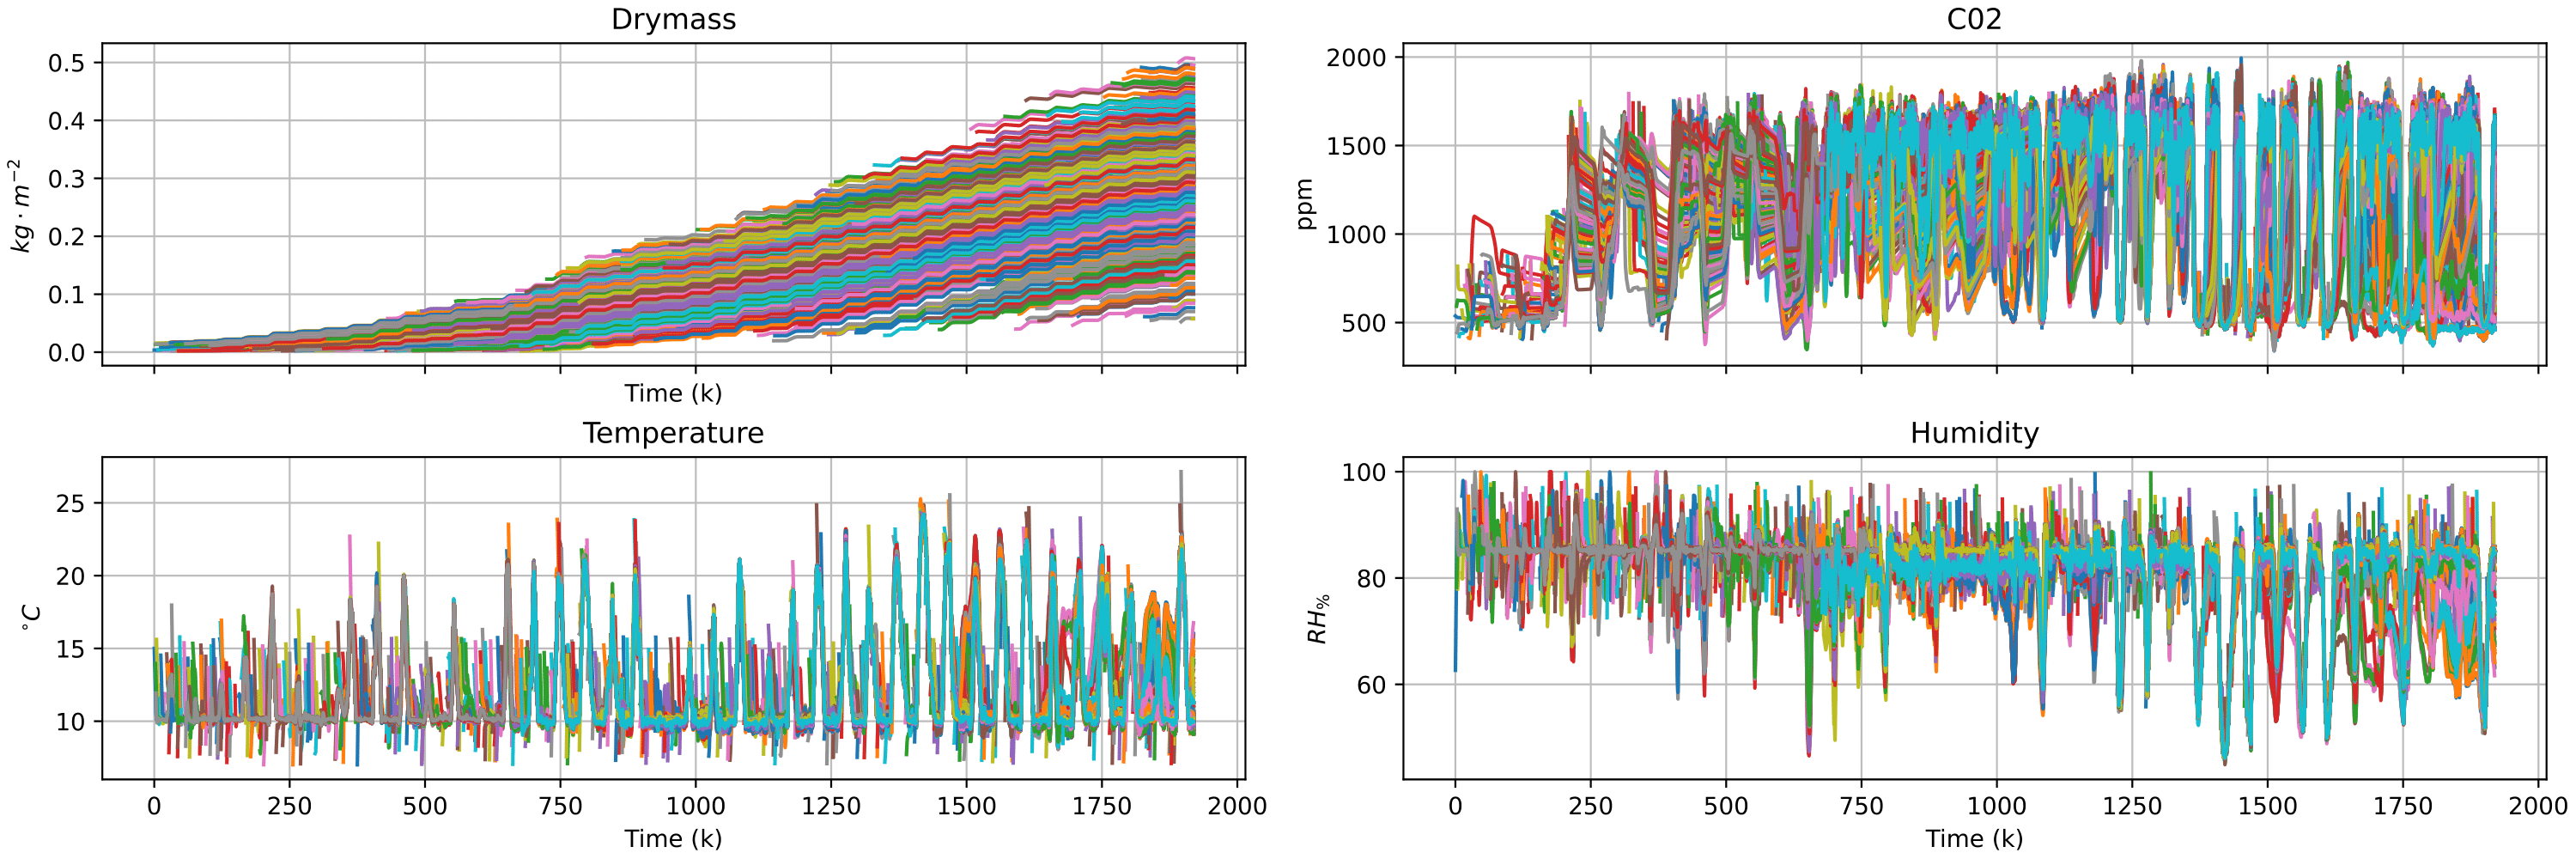
\includegraphics[width = \textwidth]{figures/sampled_states_TR-eps-converted-to.png}
    \caption{Sampled states}
    \label{fig:sampled-states-TR}
\end{figure}


\begin{figure}[H]
    \centering
    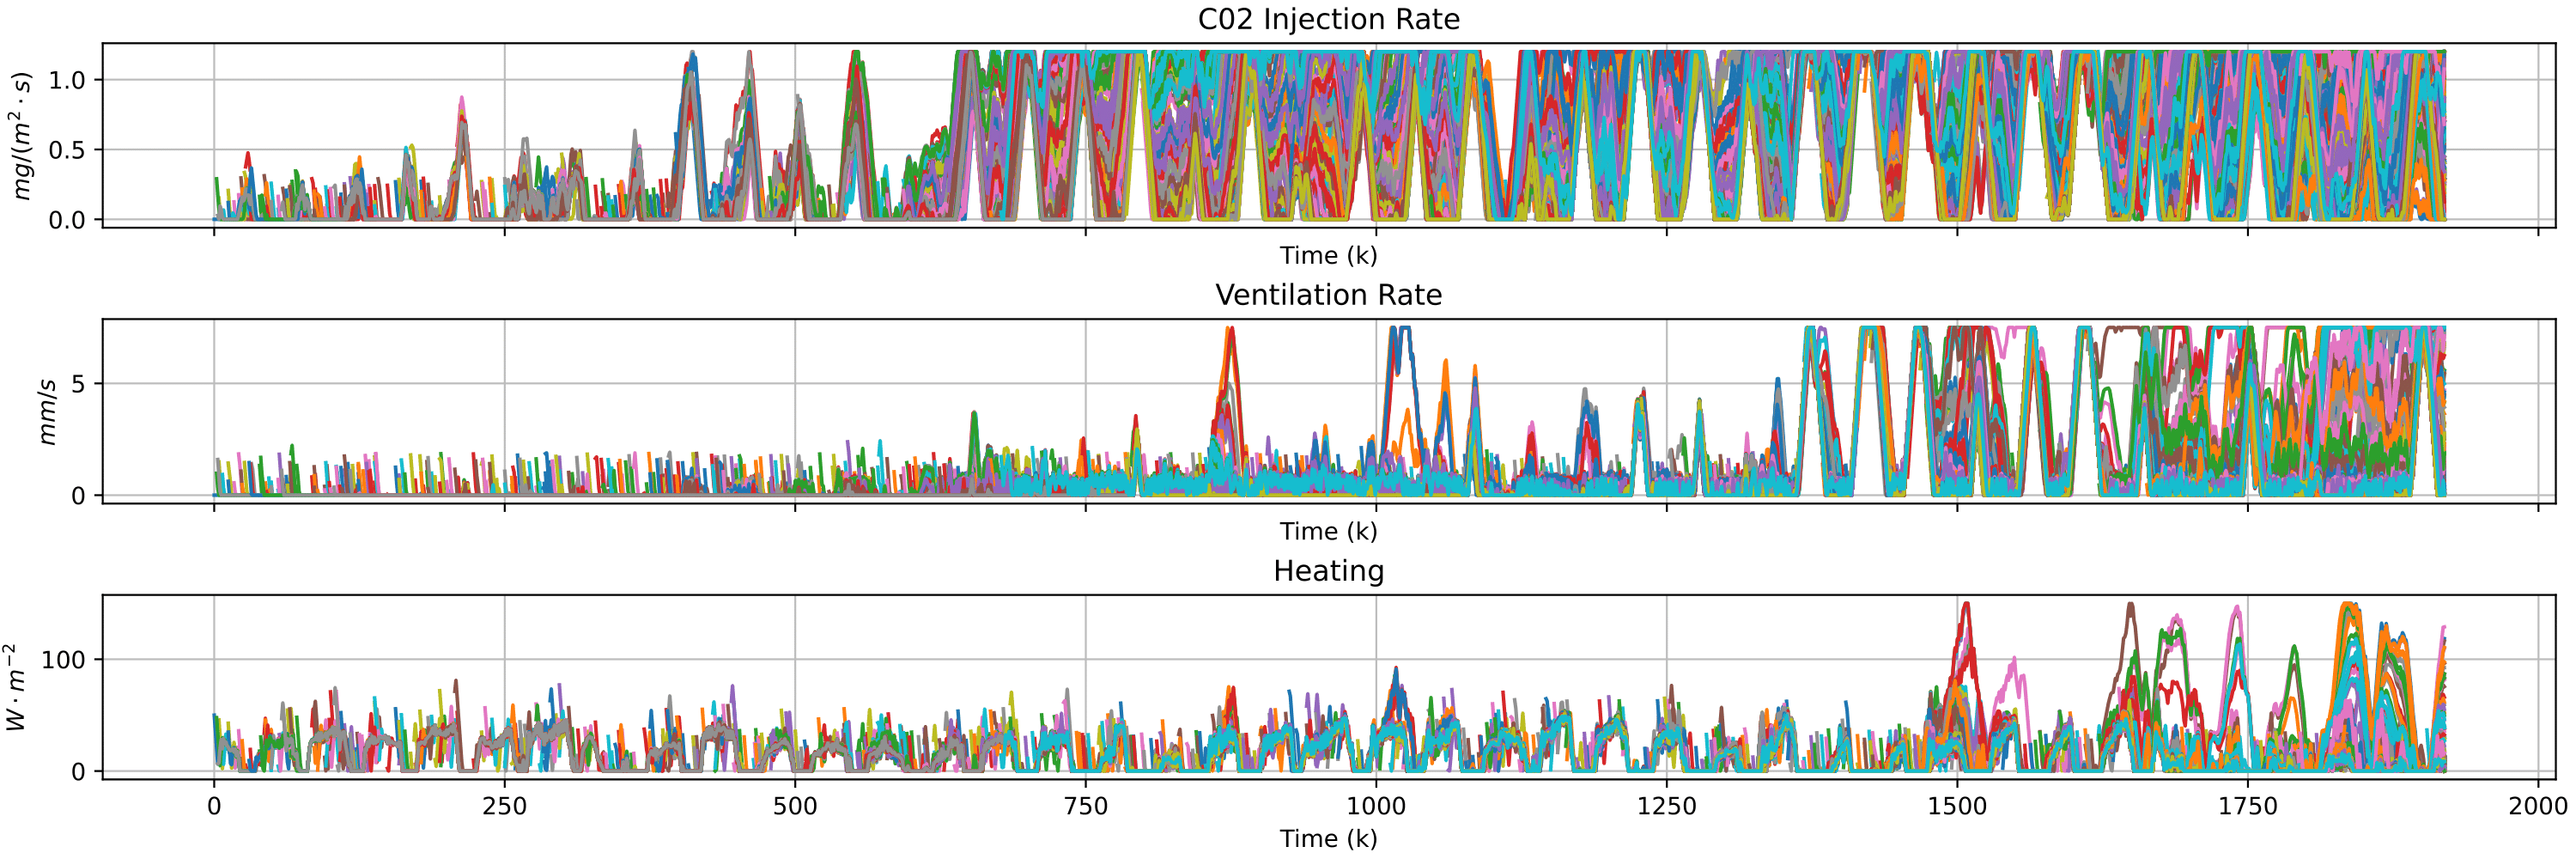
\includegraphics[width = \textwidth]{figures/sampled_inputs_TR-eps-converted-to.png}
    \caption{Sampled inputs from nominal conditions}
    \label{fig:sampled-inputs-TR}
\end{figure}

\autoref{fig:sampled-states-TR} and \autoref{fig:sampled-inputs-TR} are the results of all 1000 trajectories sampled from the nominal agent. The figures reveal that the sampled trajectories exhibit less coverage of the state and input spaces than the temporal difference learning,  \autoref{fig:sampled-states-TD} and \autoref{fig:sampled-inpts-TD}. Nevertheless, a sufficient level of coverage is achieved. Following the completion of training and validation, a small number of additional trajectories will be sampled to verify the accuracy of the prediction model.

\subsection{Results}

\begin{figure}[H]
    \centering
    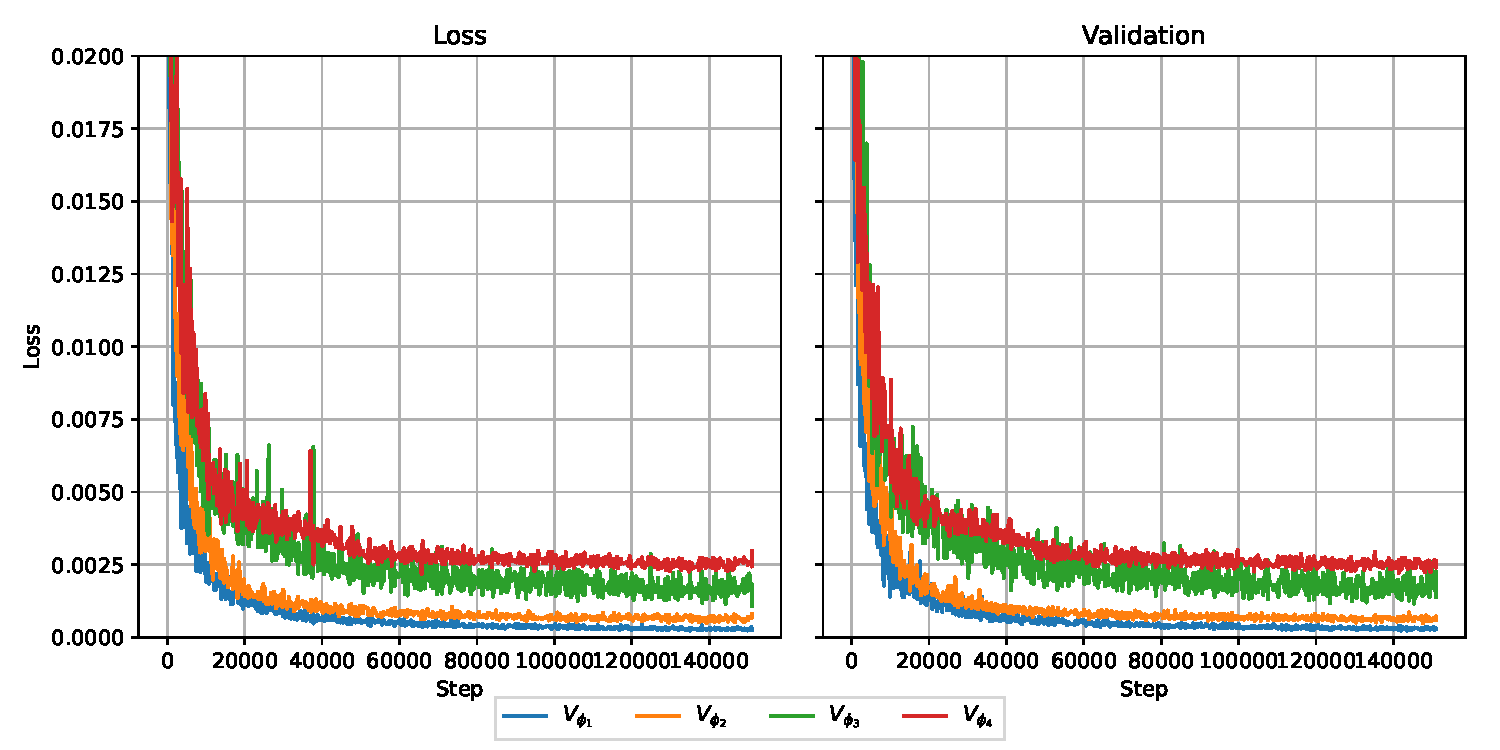
\includegraphics[width = \textwidth]{figures/tr_training_graphs.pdf}
    \caption{Performance Curves, trained on the nominal Agent}
    \label{fig:tr_perf_curves}
\end{figure}



\autoref{fig:tr_perf_curves} displays the loss curves of all four models trained on data generated by the nominal agent. As expected, the baseline model ($V_{\phi_1}$) achieves the highest accuracy compared to the simpler models. This can be attributed to its more complex structure and using the full observation returned by the agent, with each subsequent simpler model exhibiting lower accuracy. Nevertheless, when using the reduced observation space model, denoted as $V_{\phi_4}$, the model demonstrates a high level of accuracy, as evidenced by a mean squared error of less than $0.5\%$ between the actual and predicted values. The high level of accuracy indicates that the value of a state is primarily influenced by the current time and the condition of the crop’s dry mass. In addition, when incorporating these value functions into the RL-MPC framework, the optimiser would only need to optimise over two variables for $V_{\phi_4}$, as opposed to 13 variables for the other value functions.

\begin{figure}[H]
	\centering
	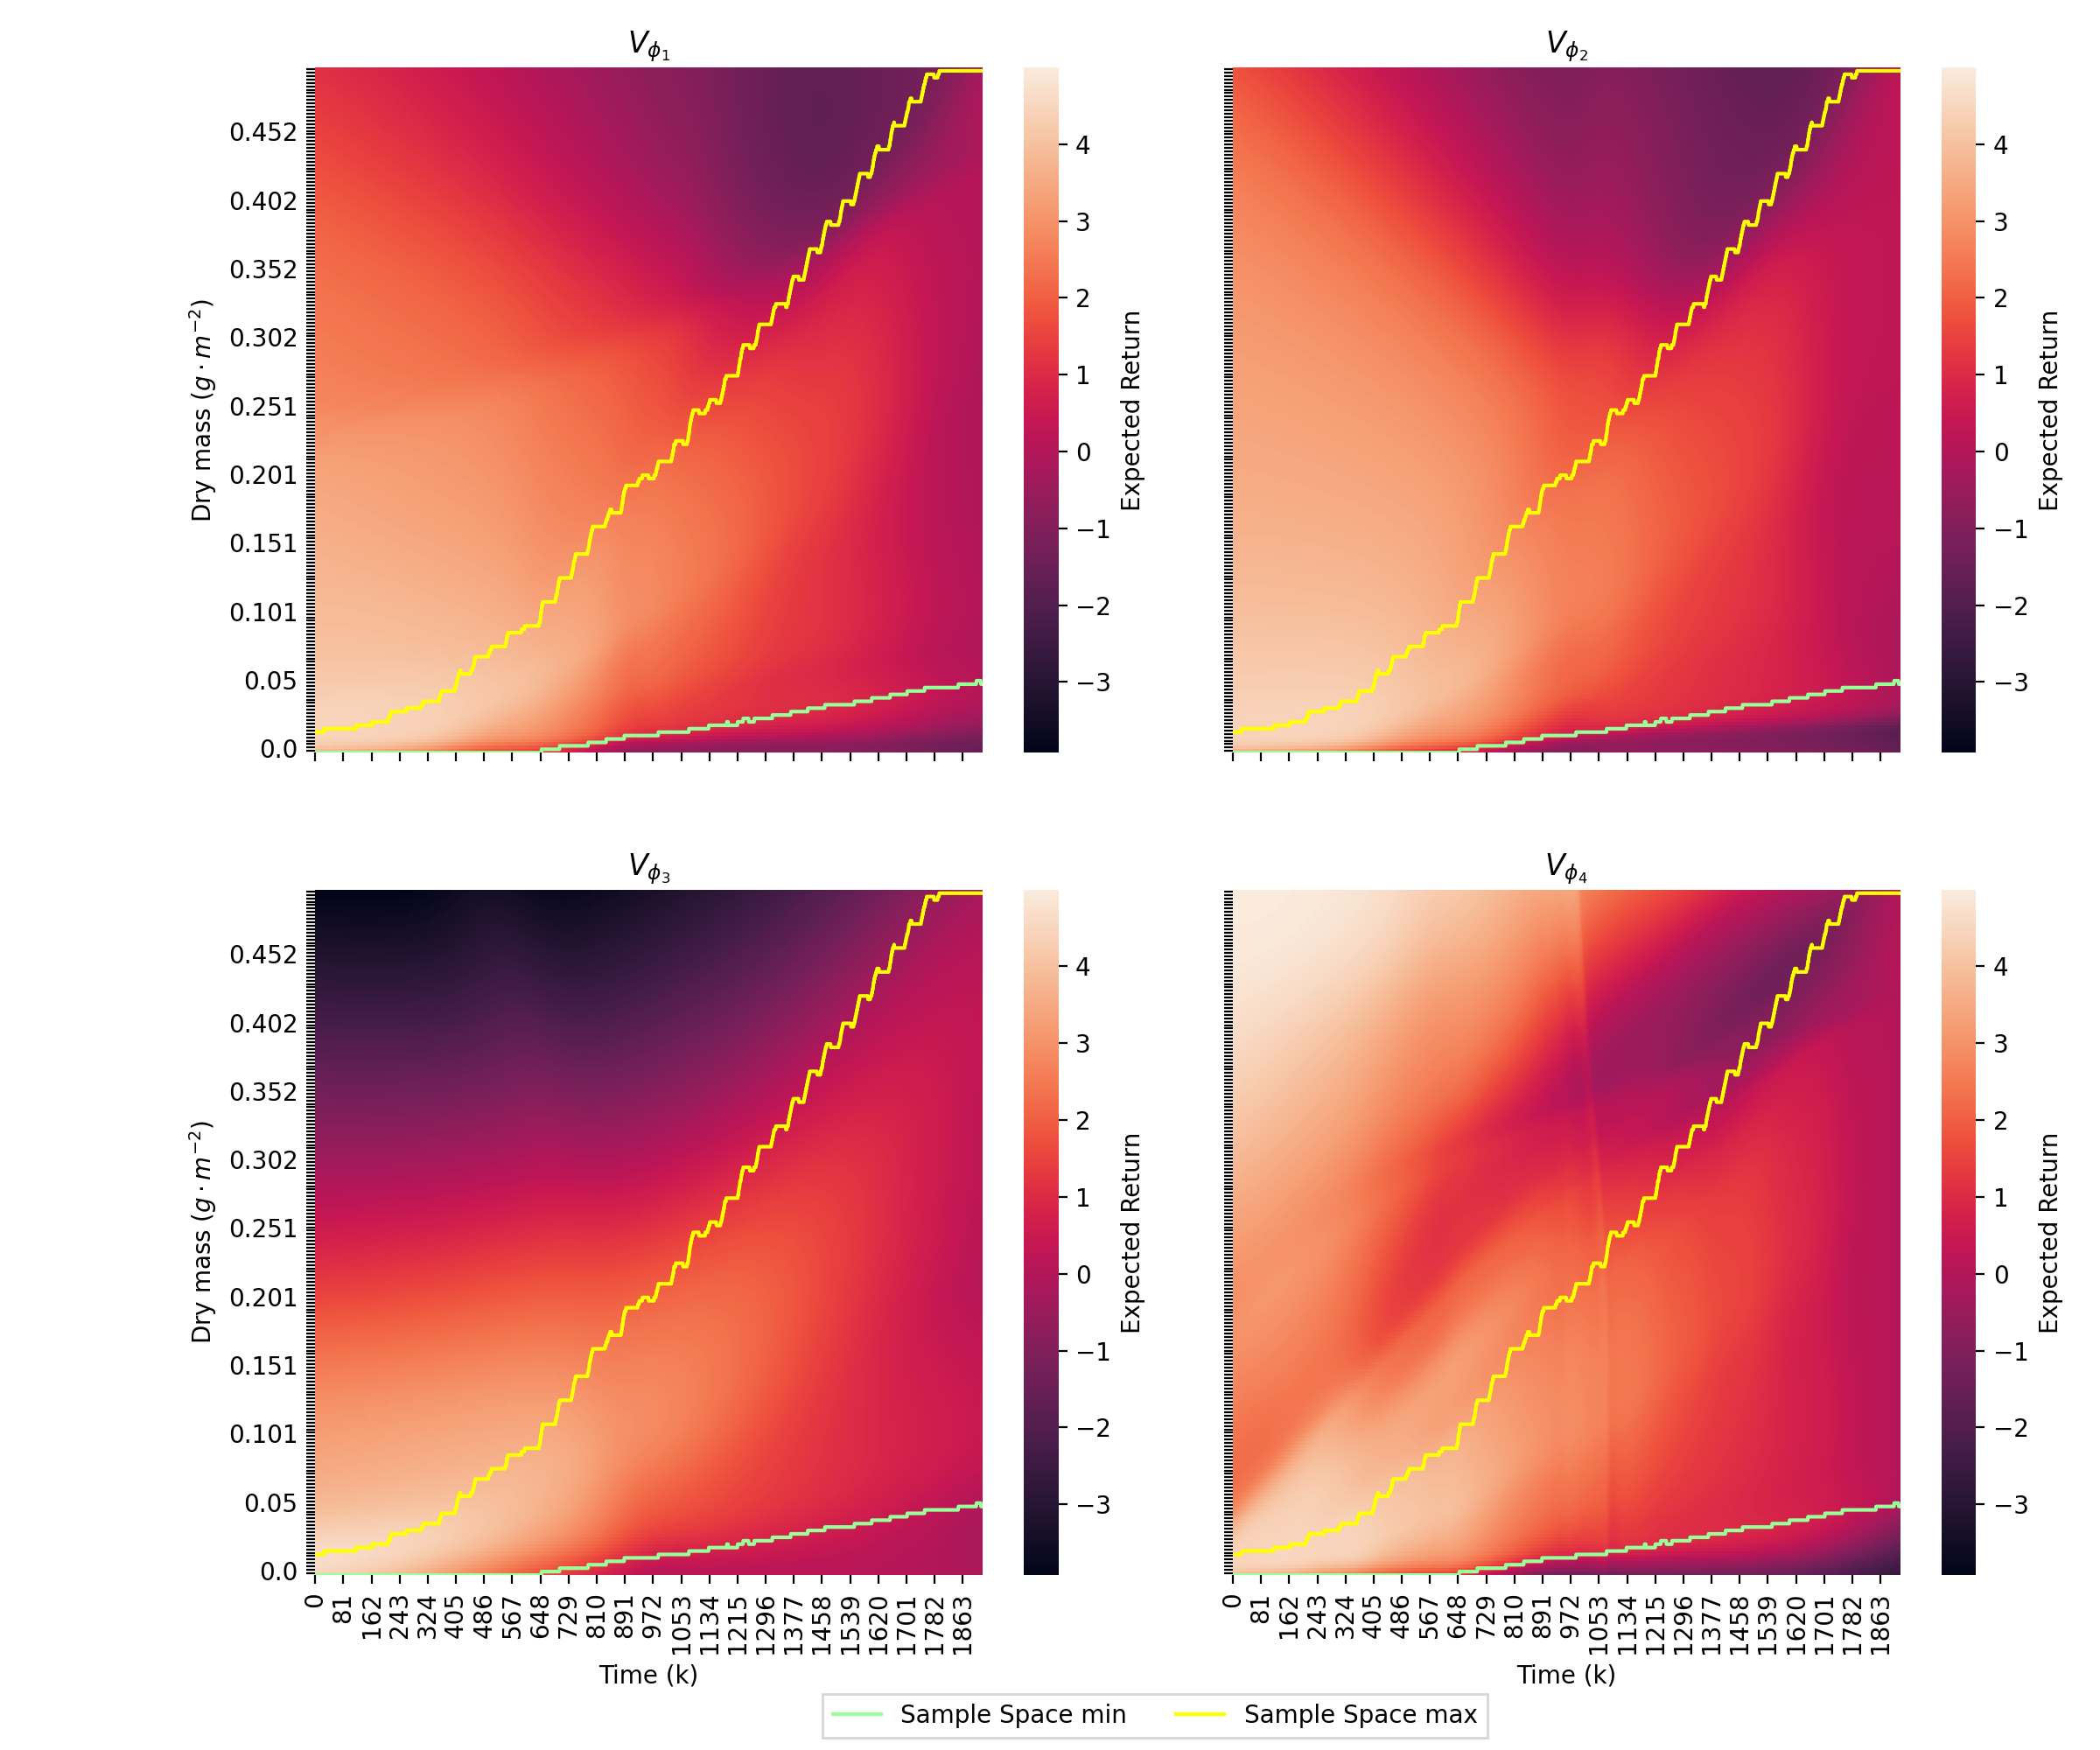
\includegraphics[width = 0.8\textwidth]{figures/vf_heatmap_deterministic.png}
	\caption{Value vs Drymass vs time}
	\label{fig:vf_heatmaps}
\end{figure}

\autoref{fig:vf_heatmaps} gives a visual representation of the value of a state given the dry mass and time. It is noted that although $V_{\phi_1},V_{\phi_2}$ and $V_{\phi_3}$ require an observation space as given in \autoref{eq:obs-tuple-1} to determine its value; since the value is mostly dependent on the dry mass state and time, the other states in the observation space were fixed and only the time and drymass were varied to produce the heatmaps as shown in \autoref{fig:vf_heatmaps}. The lower and upper limits in  \autoref{fig:vf_heatmaps} indicate the range within which the value function approximator can be deemed reliable. This range corresponds to the portion of the sample space from which the dry mass was sampled for training, i.e. this corresponds to the maximum and minimum dry mass trajectory as seen in \autoref{fig:sampled-states-TR}.

The intuitiveness of \autoref{fig:vf_heatmaps} stems from the fact that the highest expected return is observed at the beginning of the growing period, which can be attributed to its longer growing duration. It is noted that the reward function is determined by the difference in growth. Consequently, the return is calculated based on the difference in growth between an initial and end state and the energy costs incurred to achieve this growth difference. Moreover, at a given time, having a higher dry mass leads to greater expected return, specifically in the first half of the growing period. This behaviour is seen across all four models within the training bounds. It is important to note that the greenhouse model limits the dry mass to a maximum of $400 g \cdot m^{-2}$. Consequently, there will be minimal expected return for dry masses near this value. Although the nominal agent will make efforts to grow the plant by supplying carbon dioxide and heat, it will not result in any growth hence the lower returns in \autoref{fig:vf_heatmaps}.  It is also noted that \autoref{fig:vf_heatmaps} suggests that the value function is smooth concerning the dry mass and time.

\begin{figure}[H]
	\centering
	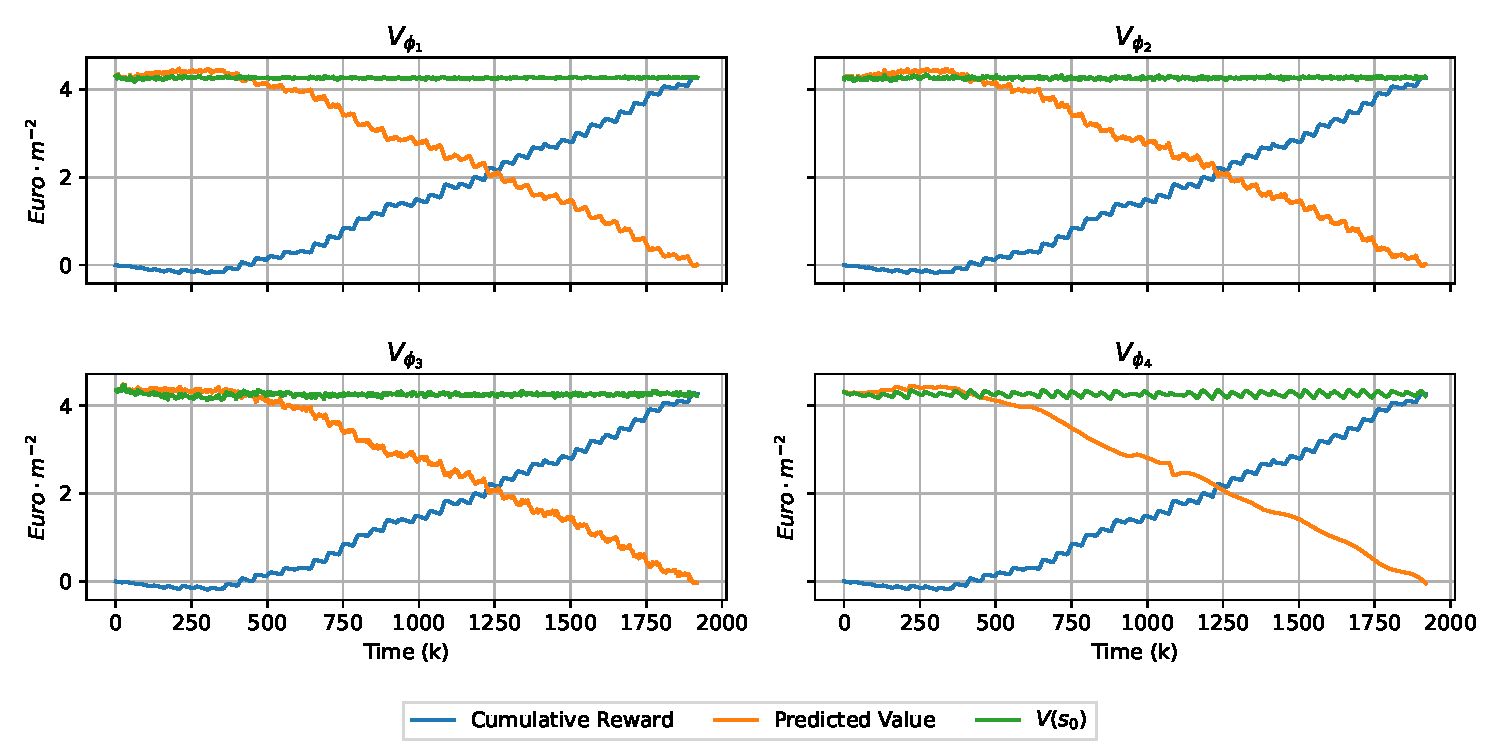
\includegraphics[width = \textwidth]{figures/vf_time_predictions_long.pdf}
	\caption{Value predictions - Entire Time Horizon}
	\label{fig:tr_predictions_long}
\end{figure}

\autoref{fig:tr_predictions_long} displays a time series plot of the cumulative rewards plotted against the predicted value at each time step over the entire simulation period. This plot is similar to that shown in \autoref{fig:vf-vs-gamma}. Additionally, it includes the calculated $V_\pi (s_0)$ at each time step using \autoref{eq:v0} as a visual indicator of the accuracy of the value function. As demonstrated in \autoref{fig:tr_predictions_long} in conjunction with \autoref{fig:tr_perf_curves}, the predicted values show a high level of accuracy. This is evident from the nearly perfect horizontal line at $V_\pi (s_0)$ that spans across the growing period and substantially outperforms the prediction accuracy of the trained value functions in \autoref{fig:vf-vs-gamma}. However, what is interesting and cannot be seen in \autoref{fig:vf_heatmaps} but in \autoref{fig:tr_predictions_long} are the fluctuations present in each prediction. Naturally, $V_{\phi_4}$ is not able to make a precise prediction of the value since it only gets the time and dry mass as inputs, however its prediction is much smoother than all the others. While $V_{\phi_1}$, $V_{\phi_2}$, and $V_{\phi_3}$ may provide more accurate predictions, they exhibit greater fluctuations. This highlights a higher degree of non-linearity. Moreover, this observation again suggests that the primary factors determining the value of a state are its dry mass and time. Meanwhile, minor fluctuations in rewards and expected returns are influenced by other factors that have minimal impact over the entire growing period.



\begin{figure}[H]
	\centering
	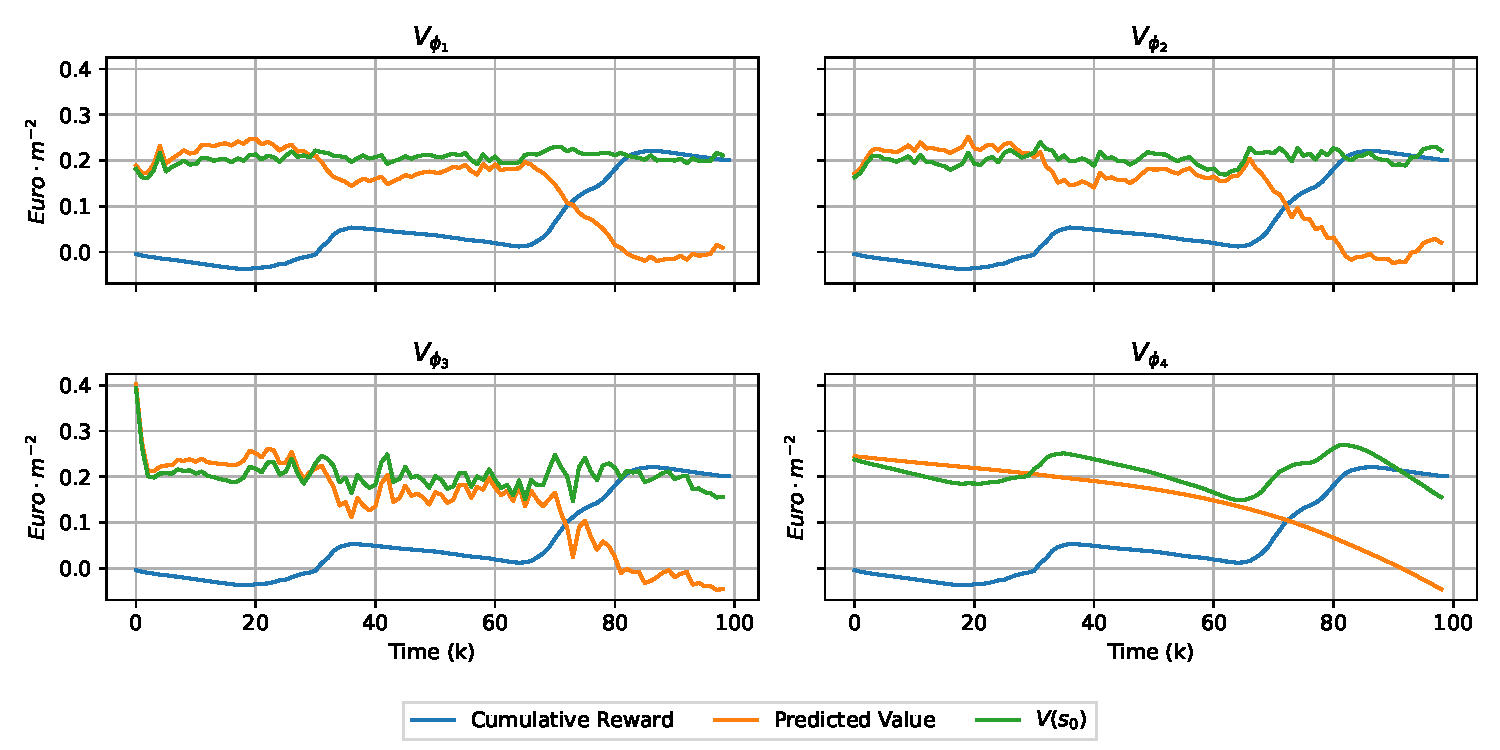
\includegraphics[width = \textwidth]{figures/vf_time_predictions_short.pdf}
	\caption{Value predictions - 2 Days}
	\label{fig:tr_predictions_short}
\end{figure}

	


\autoref{fig:tr_predictions_short} shows a time series of the cumulative reward and predicted values over two days.
 

\begin{remark}\label{rem:vf-smoothness}
	It is evident that, while $V_{\phi_1}, V_{\phi_2}, V_{\phi_3}$ can produce more precise estimations (as demonstrated by the proximity of their prediction line $V_{\pi}{s_0}$ to the actual value), $V_{\phi_4}$ remains significantly smoother. Moreover, $V_{\phi_3}$  is not as smooth as it may have seemed in \autoref{fig:vf_heatmaps} and displays the highest level of fluctuations across the four models trained. Although this is one realisation of a trajectory, this behaviour was observed in all simulated trajectories. This behaviour should be noted since it is important for integrating it with MPC due to the non-linearity of the value function.
\end{remark}



\begin{figure}[H]
	\centering
	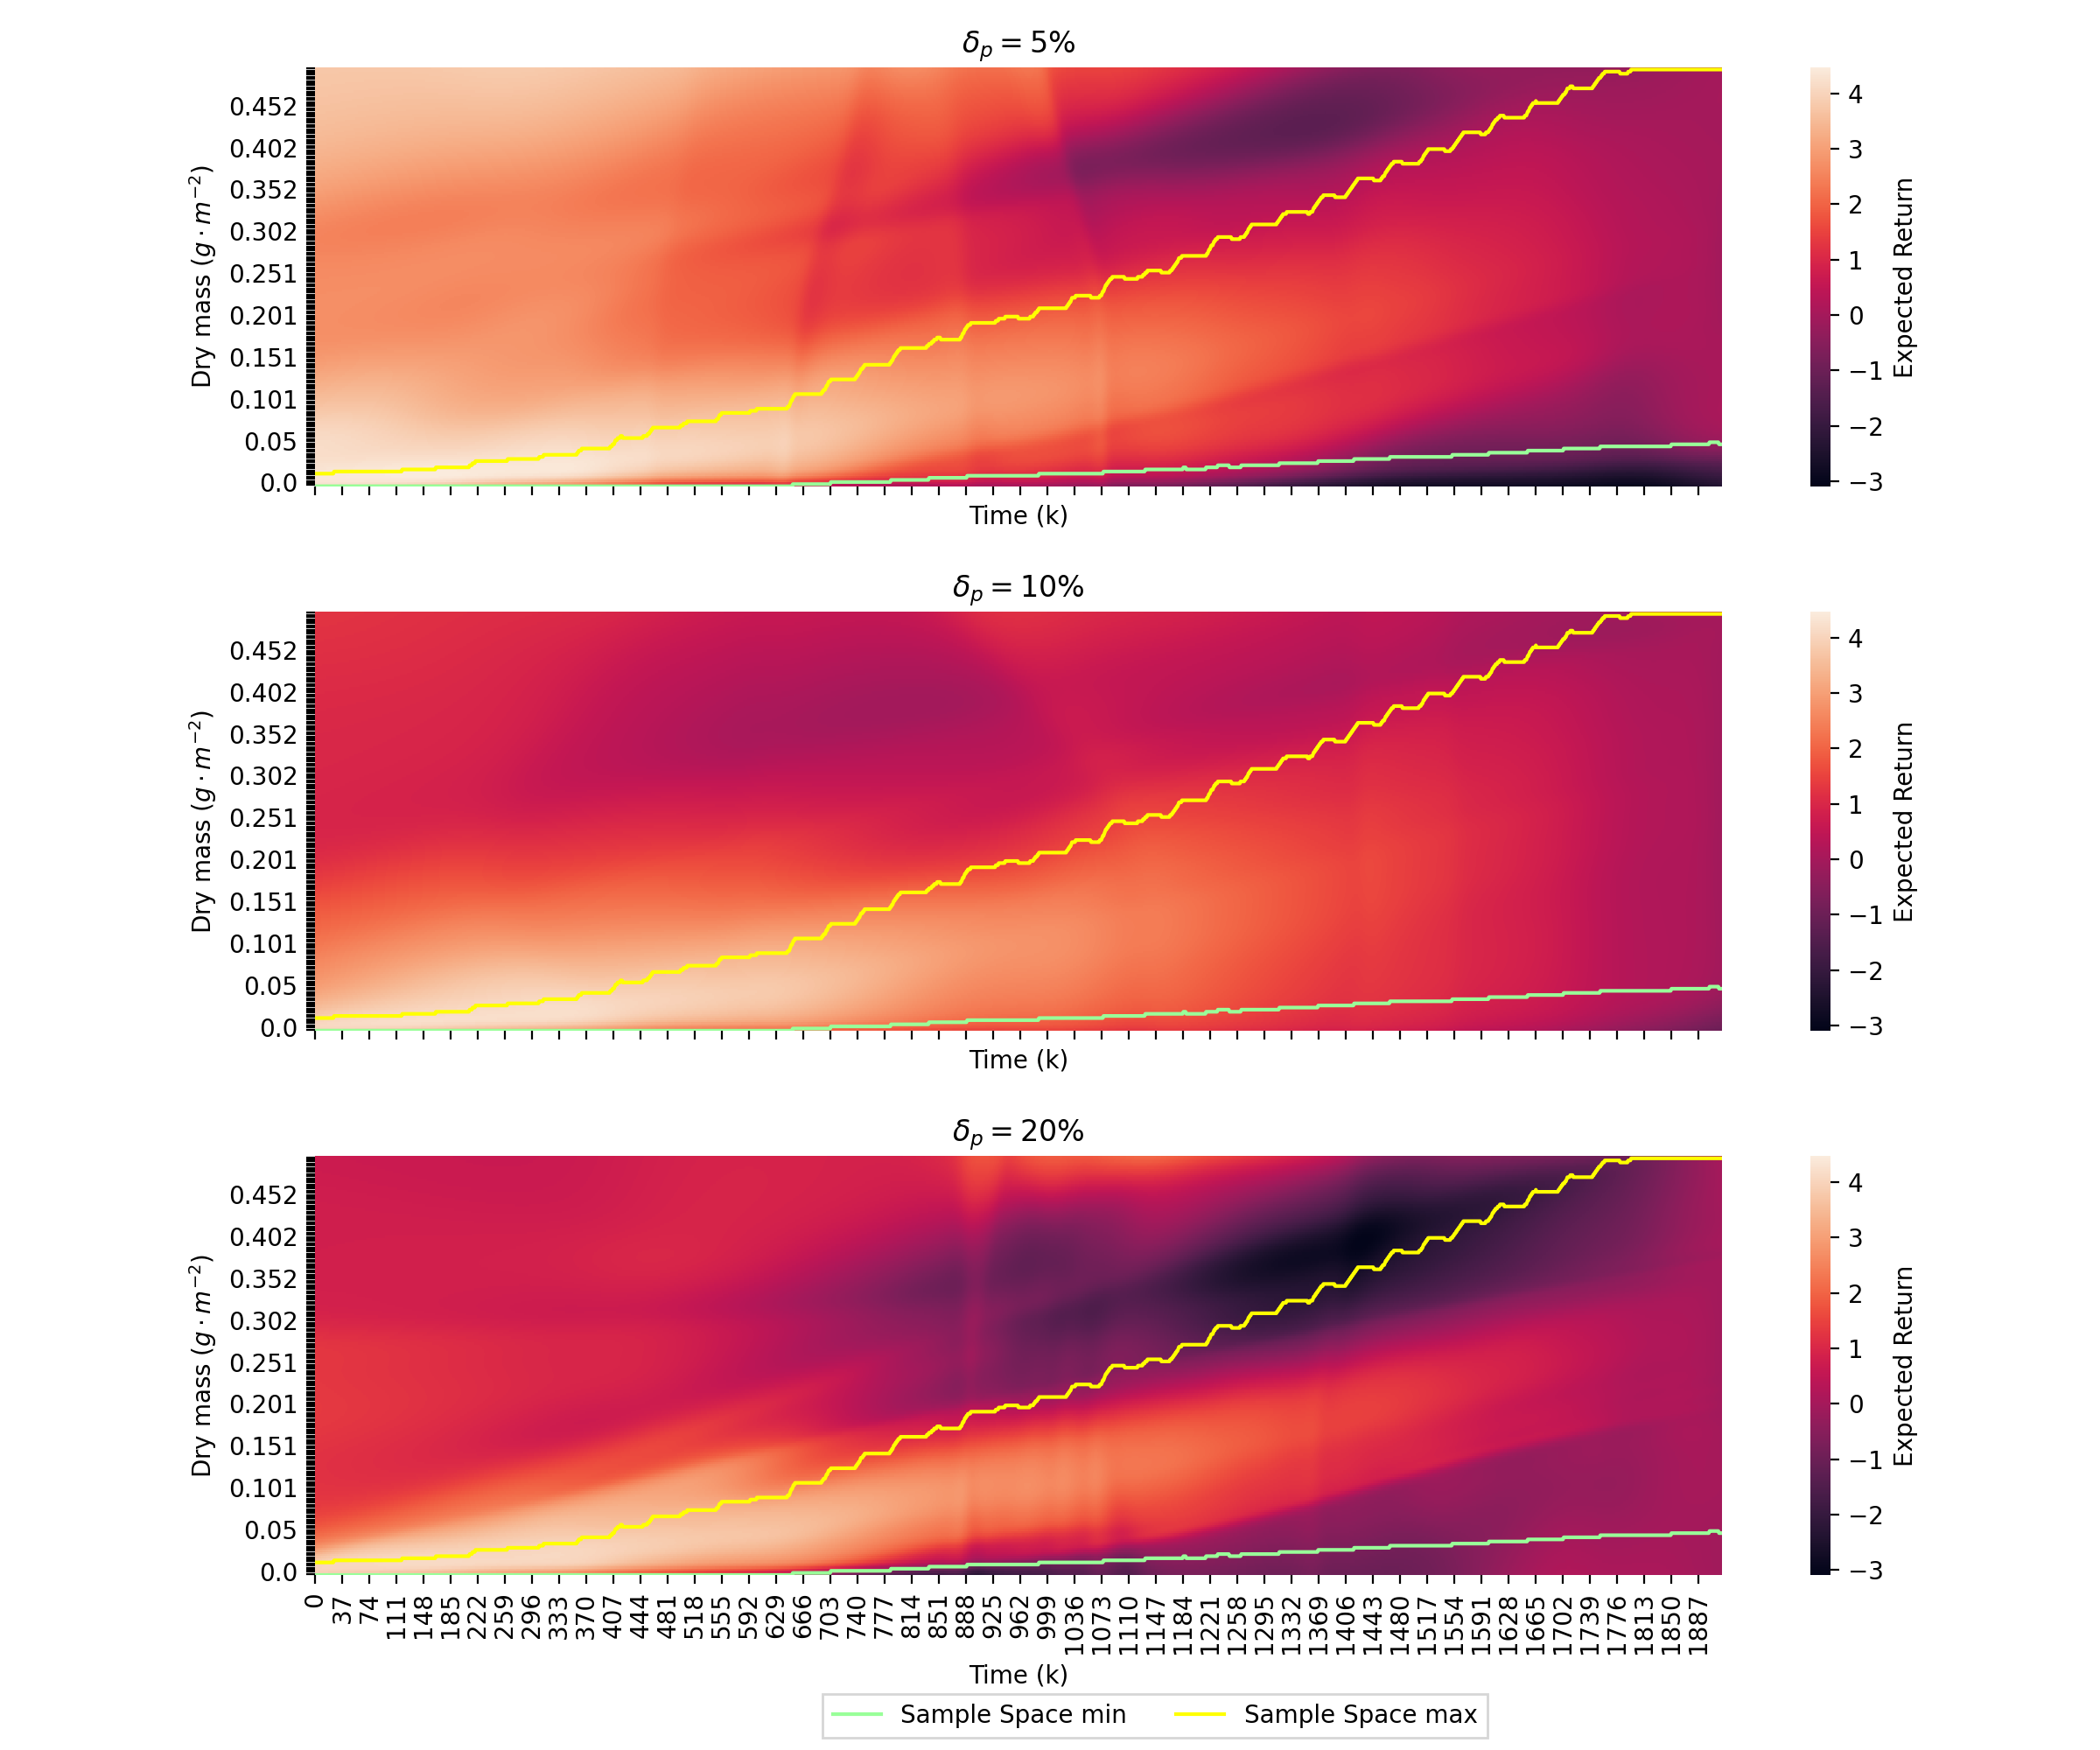
\includegraphics[width = \textwidth]{figures/vf_heatmap_stochastic_test.png}
	\caption{Drymass vs Time vs Value - Stochastic}
	\label{fig:vf_heatmap_stochastic}
\end{figure}


Finally, a value function was trained with its corresponding agent for each level of uncertainty in the environment. \autoref{fig:vf_heatmap_stochastic} displays the same heatmap as \autoref{fig:vf_heatmaps}, yielding similar behaviour compared to the nominal conditions. However, it appears to be more coarse, particularly beyond the range of the training data. Specifically, it seems that, for high uncertainties i.e. $20\%$), the trained value function exhibits a higher degree of non-linearity than the others trained on lower levels of uncertainty. This may indicate that more sample trajectories are required for further training; however, it still seems to generalise well in the region of the nominal trajectory.

The `folds' in exhibited in \autoref{fig:vf_heatmap_stochastic}, especially prevalent for $\delta = 5\%, \delta = 20\%$, is seen to appear in the middle of the growing period. This if further seen in \autoref{fig:tr_predictions_long} for $V_{\phi_4}$ where the same `folds' in the expected return can be seen in the time series. This suggests that for this brief time period, the expected return can be very accurately predicted by only the time and current dry mass. However, this could also be attributed to the poor generalisation of the value function in that specific area, which is caused by the limited availability of data for that particular region.

Moreover, for $\delta = 20\%$ in \autoref{fig:vf_heatmap_stochastic}, it seems that towards the end of the growing period and for lower dry masses, the expected return suddenly drops. This suggests a lack of training data for that region. Sampling the necessary trajectories for highly stochastic environments can be difficult, necessitating a larger number of trajectories to be sampled in order to achieve the desired data spread. However, the value function still generalises well around the nominal trajectory and was therefore deemed satisfactory.


\section{Conclusion}
The objective of this chapter was to develop a policy that is competitive with MPC and a value function that can accurately approximate the expected return given the state of the environment, both for the nominal and stochastic environment.
It was discovered that a policy trained with a discount factor of 1 resulted in a critic that provided inaccurate value estimations and a policy that performed worse than an agent trained with lower discount factors. While reducing the discount factor leads to improved policies and a more precise critic, the critics fail to provide information about the entire growth period. Furthermore, the critic must be differentiable in order to integrate the critic with MPC. This requires the use of the tanh activation function. However, using this activation function leads to a less effective policy than using a non-differentiable activation function like ReLu.

Given these obstacles, it became evident that additional measures were necessary. It was decided to train a separate critic/value-function on the best RL policy obtained. Therefore, lower discount factors and non-differentiable activation functions may be used in the policy training. The best policy found and trained on the nominal data was denoted as Agent 1 and later referred to the nominal agent, with parameters shown in \autoref{tab:selected_agents}. Using the same hyper parameters as Agent 1, three different agents were learned based on each level of uncertainty in the greenhouse model, namely Agents 0.05, 0.1 and 0.2. 

Empirical evidence demonstrated that stochastic agents were more robust to noise compared to nominal agents. Agents trained with higher levels of uncertainty exhibited policies with reduced variance across different uncertainty levels. While overall performance decreased as environmental uncertainty increased, the decline was more gradual for agents trained with higher uncertainty. Thus, agents trained on higher degrees of uncertainty showed greater robustness across all uncertainty levels.

 After generating sufficient policies for the nominal and stochastic environments, it was necessary to train an appropriate critic/value function approximator. Four different model architectures were used to train the critics, and each model architecture became progressively less complex. Every agent, whether in the nominal or stochastic case, had a critic trained to evaluate its policy under its particular level of uncertainty. 
 
 Results showed that accurate value function approximators could be trained, provided enough data was sampled. However, although they were accurate, upon closer inspection the predictions displayed small fluctuations, which could be problematic later on when integrating the function appropriators into the RL-MPC framework. However, the simplest model architecture, trained on only the dry mass state and time, provided very smooth predictions, albeit not as accurate as the more complex models. This model architecture was used to train value function approximators for the stochastic agents. These agents and corresponding value functions established the foundation for incorporating RL with MPC into the RL-MPC framework.

